% GROUP_A_MANUAL_REPORT: this source is maintained alongside the evidence ledgers.
\documentclass[12pt,a4paper]{article}
\usepackage[margin=1in]{geometry}
\usepackage{iftex}
\ifPDFTeX\usepackage[T1]{fontenc}\usepackage[utf8]{inputenc}\usepackage{mathptmx}\else\usepackage{fontspec}\setmainfont{Times New Roman}\fi
\usepackage{longtable,booktabs,array,enumitem,microtype,xcolor,needspace}
\usepackage{tikz}
\usetikzlibrary{arrows.meta}
\usepackage[hidelinks]{hyperref}
\usepackage{parskip}
\setlength{\emergencystretch}{3em}
\setlist{nosep}
\newcolumntype{P}[1]{>{\raggedright\arraybackslash}p{#1}}
\newcommand{\pending}[1]{\textcolor{red}{#1}}
\title{GPU Sharing Mechanisms for Multi-Tenant Inference Serving\\\large Group A: Search Execution and Evidence Report}
\author{MUHAMMAD BURHAN UN NADEEM (SE-24071)\\MUHAMMAD FAAIZ ALAM (SE-24094)\\ALI RAZA (SE-24302)}
\date{17 October 2026\\Operating Systems Complex Engineering Problem\\NED University of Engineering and Technology}
\begin{document}
\maketitle
\begin{abstract}
This intermediate deliverable records execution of the submitted SLR protocol and prepares traceable evidence for the final CEP report. The 11 October IEEE/Springer checkpoint contains 689 formal query occurrences and 21 accepted studies. A 14 October extension supplied 23 ACM/ScienceDirect export files with 3,727 parsed occurrences. A supplied 17 October screening register resolves 585 formerly open occurrence decisions and audits assisted exclusions. An interim four-source PRISMA stage map now balances the captured populations while identifying four proposed links and open retrieval cases; \pending{the canonical CSV/workbook and final report-level flow still require reconciliation.} Batches 1--3 assess 31 supplied queue reports: 22 accepted and nine excluded. Batch 3 adds nine accepted studies and excludes one training-only report. The current accepted set is 43. Source-anchored reviews and receipts are integrated separately from the historical flow. Run-count discrepancies and remaining extraction gaps remain explicit.
\end{abstract}
\textbf{Status: evidence checkpoint, not final SLR.} The publication window is 1 January 2020--11 October 2026 inclusive. One AI reviewer conducted screening and appraisal at the user's direction; the listed students are the project authors, not claimed independent reviewers. \pending{Red text identifies statements, counts or conclusions that must be revisited when the remaining search reconciliation, screening, QA and extraction work is completed.}
\newpage\tableofcontents\newpage
\section{Purpose and requirements}
The engineering problem is to share a physical GPU among inference tenants while balancing useful work and density against predictable latency and isolation. The assigned alternatives are time-slicing, MPS, MIG and API remoting/virtualization, including hybrids. The unit of technical comparison is local sharing on one GPU. A study containing cluster experiments qualifies only when local inference-sharing evidence is identifiable; cluster-wide GPU counts are never substituted for local occupancy.

The submitted \texttt{report/SLR\_protocol.tex} and \texttt{report/SLR\_protocol.pdf} are the protocol baseline identified by the user. The protocol contents are preserved. Query deliverables reside in the root \texttt{report/} folder; Group A evidence remains under \texttt{groups/group-a/evidence/}. The final assignment still requires 15--20 unique peer-reviewed primary studies, at least 15, a 12-point IEEE-cited LaTeX report, and approximately 20--30 pages of main content. Meeting a provisional paper count does not complete searching or the final deliverable. No additional intermediate-page requirement was supplied.

The five questions ask which mechanisms are evaluated (RQ1), how outcomes are measured and compared (RQ2), which operating conditions change results (RQ3), what trade-offs and gaps remain (RQ4), and what conditional choice is supported (RQ5). All five map to extraction and the claim register, rather than to an unconditional ranking of mechanisms.

\section{Protocol adoption and deviations}
The Group A execution copy adopts the submitted protocol. Amendment GA-A001 extends the cutoff from 27 September to 11 October 2026. GA-A002 records the user's instruction that Codex conduct screening and quality appraisal as a single AI reviewer. There is no independent second reviewer, inter-rater agreement statistic or adjudicated human consensus. GA-A003 permits supplementary full-text work while unavailable database coverage remains open. GA-A004 records the actual public-interface execution and metadata capture in place of signed-in publisher exports. None changes the inclusion criteria to meet a target count.

Eligibility requires an English peer-reviewed original journal or full conference report, a local sharing/partition/process/API mechanism, explicit concurrent inference or justified mixed inference evidence, and sufficient configuration/outcome detail. Training-only, cluster-only, surveys and vendor claims are excluded from the primary set. Unretrieved reports are pending access outcomes, not assessed full-text rejections. Related conference, journal and preprint reports are one underlying study until an independent contribution is established.

% Detailed reporting of Group A's adopted protocol and executed evidence stage.
\section{Review design and operational definitions}
\label{sec:review-design}
This report is the execution record for the adopted Group A protocol, not a second protocol. The decision unit is a unique evaluation of concurrent inference sharing on a physical GPU. An imported search hit is an \emph{occurrence}; matching occurrences are linked to a canonical bibliographic record; a publication version is a \emph{report}; and related reports can describe one \emph{study}. These units are kept separate in every table and flow count. In particular, a server-level GPU saving or an eight-GPU placement outcome cannot be presented as a one-GPU utilization measurement merely because the same paper also evaluates local sharing.

\begin{longtable}{P{0.09\linewidth}P{0.45\linewidth}P{0.36\linewidth}}
\toprule RQ & Analytic question & Evidence needed\\\midrule\endhead
RQ1 & Which temporal, MPS, MIG, API/runtime and hybrid controls were evaluated? & Mechanism, control layer, local tenant arrangement and comparator.\\
RQ2 & Which outcomes and experimental methods make results comparable? & Metric definition, units, percentile/SLO, denominator, measurement window and baseline.\\
RQ3 & Which workloads, hardware and configurations change the outcome? & GPU/SKU, profile/quota, model and batch, arrivals, co-tenant mix and resource pressure.\\
RQ4 & What engineering costs, isolation properties and contradictory observations are supported? & Within-paper trade-offs, limitations, resource/fault/security experiments and counterexamples.\\
RQ5 & Under which operating requirements is a choice supported? & Conditional synthesis with direct/indirect evidence and explicit unresolved conditions.\\
\bottomrule\end{longtable}

The main window is 1 January 2020 through 11 October 2026 inclusive. The publisher's broad 2020--2026 year filter is a retrieval aid; exact dates near the cutoff require checking at the report level. An older seminal exception requires a documented reason in the eligibility record. A result published after the cutoff is not made eligible by appearing in a later export. \pending{The exact-date decisions for potentially relevant 2026 reports in the new exports remain to be completed.}

\subsection{Eligibility decisions and source type}
An included primary study must be an English peer-reviewed original journal or full conference report with identifiable concurrent inference evidence, a relevant local GPU-sharing control, and enough configuration and outcome detail to evaluate the research questions. Mixed inference/training studies can contribute only when the inference outcome is separable. Surveys and vendor descriptions may explain terminology but cannot supply an included primary experiment. Reports that cannot be retrieved remain access cases.

At full text, the adopted protocol records one principal reason, with secondary notes where helpful. E1 denotes no inference-serving evidence; E2 no relevant single-node multi-tenant sharing; E3 a mechanism outside scope; E4 training-only; E5 cluster orchestration without separable local sharing; E6 no peer-reviewed original primary report; E7 insufficient technical or outcome detail; E8 a duplicate or less complete report of the same study; E9 a date/language violation without exception; and E10 another written reason. A code is assigned after reading the relevant full report, not inferred from the publisher hit count. \pending{The final distribution of full-text reasons will be recalculated after the new reports are assessed.}

\section{Database-specific search implementation}
\label{sec:search-detail}
\newcommand{\MasterQuery}{\begingroup\footnotesize\ttfamily (GPU OR "graphics processing unit") AND (inference OR "model serving" OR "deep learning" OR DNN OR LLM) AND ("time slicing" OR "time sharing" OR "context switching" OR MPS OR "multi-process service" OR MIG OR "multi-instance GPU" OR "GPU partitioning" OR "API remoting" OR "CUDA remoting" OR "GPU proxy" OR "GPU virtualization")\endgroup}
The four NED-listed platforms cover engineering journals, computing proceedings and related systems literature, but their interfaces differ in fields, syntax and export behavior. The submitted protocol's common concept block combines GPU terminology with inference/model-serving terminology; the mechanism block covers the assigned families. The recorded executed strings, rather than a retrospectively improved expression, define what was searched. The old five runs and the five later successful runs are separate dated executions. Blocked pilots are retained as attempts with no countable retrieved population.

\begin{longtable}{P{0.17\linewidth}P{0.43\linewidth}P{0.30\linewidth}}
\toprule Platform and family & Executed expression structure & Field/filter and consequence\\\midrule\endhead
IEEE MPS, MIG, temporal, API & \texttt{(GPU OR "graphics processing unit") AND (inference OR "model serving" OR "deep learning" OR DNN OR LLM) AND} one family block. & All metadata; 2020--2026. The public implementation was not the planned field-qualified Command Search.\\
Springer master & \MasterQuery & General search; English, Research or Conference Paper, 2020--2026. Full-text/reference indexing broadens irrelevant matches.\\
ACM master & \MasterQuery & All Fields, E-Publication Date 2020--2026; logged Full-Text Collection. Export page overlap/coverage is unresolved.\\
ScienceDirect temporal, MPS, MIG, API & \texttt{(GPU OR "graphics processing unit") AND (inference OR "model serving" OR "deep learning") AND} one family block per run. & The master exceeded the connector limit. The fallback omits DNN/LLM and is not equivalent to the other platforms' common block.\\
\bottomrule\end{longtable}

The Springer and ACM cells reproduce their identical entered master expression in full. ACM's displayed version wraps each term in an All Fields expression and adds an E-Publication Date clause; the exact transformed string is retained in \path{search_runs_received.csv}. The IEEE and ScienceDirect cells summarize four family expressions each; their verbatim run-specific strings, source URLs, hits and export receipts are retained in \path{search_runs.csv}, \path{search_runs_received.csv} and \path{export_intake.csv}. The ACM two-file overlap and the ScienceDirect MPS re-export show why a parsed-row count is not itself evidence of complete page coverage. The temporal URL's Open Access facet is documented separately from the unfiltered count observed later. \pending{The final search-coverage statement depends on the ACM export decision, verified filter provenance and any justified amendment; no missing-hit number is imputed.}

A 17 October provenance review of an uploaded zip confirmed that all 23 included export files match the receipt ledger by hash and size, and found no screenshot or page-range record in that zip. The zip's file times appear to reflect a later copy and cannot establish the original export times. The helper's separate folder and the live PC directory have not been checked in this review. The two ACM files contain 829 and 1,000 entries with 442 repeated exact keys; overlap suggests page ranges may have intersected, but neither the original ranges nor any number of omitted results is known. \pending{The team must record a dated decision to re-export ACM in traceable chunks or retain this coverage limitation.} The original run log is preserved, with its received copy differing only by a final CRLF. No query, log or export has been retrospectively changed to reconcile the site counts.

\section{Selection, identity and PRISMA accounting rules}
\label{sec:accounting-rules}
Every imported occurrence retains its source file, run and stable ID. An exact DOI or key can propose a link, while a normalized title with a different DOI triggers version review rather than automatic deletion. A conference paper, journal extension and preprint can be several reports of one study. The most complete peer-reviewed report is preferred for claims, while the related versions remain in the history. Whole-proceedings volumes and books in the ACM export need an explicit non-primary-record treatment; their bibliographic keys do not make them individually evaluated papers.

The 11 October checkpoint demonstrates the arithmetic for its captured subset: 689 formal occurrences minus 10 duplicate occurrences plus 20 selected supplementary records yields 699 records considered; 575 earlier-stage exclusions and 96 pending/not-retrieved cases leave 28 assessed reports; seven report-level exclusions leave 21 unique accepted studies. This is a dated checkpoint, not the final four-database flow. A subsequent review note checks all 515 exact DOI/key links, supplies one missing canonical target, and identifies four chains, while the current CSV has not yet been updated. The Step 5 note revises the first-pass classes to 515 repeats, four additional links, 3,130 title/abstract exclusions and 78 advanced/assessed occurrences. These occurrence classes balance at 3,727, but they are not yet canonical report or study counts. \pending{The ledger corrections, report-version links and retrieval outcomes must be applied before constructing the merged PRISMA boxes.}

\begin{longtable}{P{0.24\linewidth}P{0.57\linewidth}}
\toprule Stage & Reconciliation rule and required ledger evidence\\\midrule\endhead
Identification & Sum imported occurrences by database/run and supplementary route; retain source file and original display observations separately.\\
Before screening & Count adjudicated duplicate occurrences and any other removals from named occurrence-to-canonical links; do not remove a report merely for sharing a study ID.\\
Title/abstract & Count canonical records screened and exclusions with reasons; keep title-only and abstract-informed decisions distinct.\\
Retrieval & Map records advanced to reports sought; record each not-retrieved report and access attempts without treating it as an assessed exclusion.\\
Full text & Count assessed reports and one principal exclusion reason per excluded report; link multiple included reports to unique studies.\\
Inclusion & Show both included reports and unique studies, with study-to-report identity reconciled.\\
\bottomrule\end{longtable}

\pending{The final four-database PRISMA flow, its reason totals and included-study count must replace the interim figure after the new occurrence ledger is adjudicated.} The flow cannot be completed by choosing a convenient difference between a displayed publisher total and an export count. A publisher interface observation and the set of files actually received remain separate provenance facts.

\section{Quality appraisal and extraction instrument}
\label{sec:instruments}
Quality scoring is applied to eligible evidence after full-text assessment; it is not a threshold that creates eligibility. Each criterion receives 0, 0.5 or 1, with an individual rationale and source anchor. High (8--10), moderate (6--7.5) and low (below 6) are reporting/interpretability bands. A paper's score is not a security certification, replication claim or proof that its baseline is suitable for all uses.

\begin{longtable}{P{0.10\linewidth}P{0.76\linewidth}}
\toprule Item & Question scored from the report\\\midrule\endhead
Q1 & Is the engineering question and tenant setting explicit?\\
Q2 & Is the mechanism and its configuration sufficiently described?\\
Q3 & Are hardware, software and resource environments identifiable?\\
Q4 & Are workloads, arrival patterns and co-tenant conditions described?\\
Q5 & Is the comparator appropriate and its resource budget clear?\\
Q6 & Are metrics, units, percentiles and denominators defined?\\
Q7 & Are repetitions, warm-up, measurement windows and other controls adequate?\\
Q8 & Does the cited figure/table/prose support the stated result?\\
Q9 & Are validity limits and adverse cases discussed?\\
Q10 & Can the setup be reproduced or at least critically interpreted?\\
\bottomrule\end{longtable}

The extraction form links a preferred report and study ID to source type/version, GPU generation and partition or quota, driver/runtime, model and tenant mix, batching/arrival process, comparator, metric and statistic, a bounded outcome, caveat and exact source location. It distinguishes a missing transcription (\texttt{NOT EXTRACTED}) from a checked absence in the report (\texttt{not reported}). A graph with unreadable pixels is not reverse-engineered into an exact value. The first 21 rows and the two preliminary new assessments are at different maturity levels; \pending{newly eligible studies require formal QA, version linkage and a complete anchored extraction before joining the synthesis.}

\begin{longtable}{P{0.25\linewidth}P{0.59\linewidth}}
\toprule Isolation field & What the observation can and cannot support\\\midrule\endhead
Performance interference & Measured latency/throughput under specified co-tenants; cannot alone prove a security boundary.\\
Resource and memory separation & Profile/quota or memory behavior and measured contention; a partition label alone does not establish an observed guarantee.\\
Adversarial security & Explicit hostile-tenant or access-control experiment, if reported; otherwise mark not established.\\
Fault containment & Explicit failure or fault-propagation experiment, if reported; ordinary workload fairness is not a substitute.\\
\bottomrule\end{longtable}

The source-linked cards in Appendix~\ref{app:cards} give an auditable QA and extraction view for the current 21-study checkpoint. They are a compact reproduction of the Group A registers, not additional independently reviewed studies. \pending{Cards, scores and claims must be regenerated if eligibility, preferred versions or source-grounded extraction changes.}


\section{Search execution and provenance}
NED's E-Resources page lists the four planned publisher platforms. The listing was checked on 11 October 2026: \url{https://eaklibrary.neduet.edu.pk/eakl/E-Resources.html}. It confirms platform availability in the list, not entitlement to each requested article. No university credentials or licensed full-text PDFs enter this public repository.

\begin{longtable}{P{0.27\linewidth}P{0.38\linewidth}P{0.25\linewidth}}
\toprule Source/run & Actual implementation & Observed hits\\\midrule\endhead
IEEE MPS & All metadata; years 2020--2026 &25\\
IEEE MIG & All metadata; years 2020--2026 &23\\
IEEE temporal & All metadata; years 2020--2026 &45\\
IEEE API & All metadata; years 2020--2026 &9\\
Springer master & General search; English; research articles/conference papers;2020--2026 &587\\
ACM pilot (11 October) & Search blocked by challenge loop &Unknown; no import at that checkpoint\\
ScienceDirect pilot (11 October) & Search page unavailable &Unknown; no import at that checkpoint\\
\bottomrule
\end{longtable}
The common block is GPU or graphics-processing-unit AND inference, model serving, deep learning, DNN or LLM. IEEE uses one family block per run. Springer uses all family blocks in one OR group. Exact strings, filters, source URLs, dates and export limitations are in \texttt{search\_runs.csv}. The IEEE field implementation differs from the planned field-qualified Command Search and is disclosed, not described as an equivalent validated command. Research type/language and precise 2026 cutoff checks are manual where facets are unavailable. No accepted study is dated after 2025.

All 30 Springer result pages (20 hits/page,7 on the final page) and all IEEE pages were captured, yielding 587+25+23+45+9=689 occurrences. These are rendered-result metadata imports, not publisher-generated RIS/CSV exports. Springer export redirects to sign-in; IEEE results export requires personal sign-in and public citation export timed out. The imports retain IDs, database/run, page, title, DOI/URL and displayed date/item metadata. Clock time was not retained and is marked unrecorded.

Springer's broad index includes reference/full-text matches and unrelated acronym expansions such as welding MIG. Search hits therefore do not imply eligible GPU studies. Seed checks recovered ParvaGPU and KRISP in IEEE; papers in other publisher proceedings required supplementary discovery at this checkpoint. Supplementary records are selected named-paper lookups checked after adoption, including submitted seeds and related systems. They are not an exhaustive search-engine result export or completed backward/forward citation search. Their follow-up query strings are reproducible suggestions, not invented historical exact queries.

\section{14 October ACM and ScienceDirect extension}
The operator supplied 23 database export files and a search log from the named PC export directory. All 23 export SHA-256 hashes were checked against \path{export_intake.csv} on 16 October and matched. A separate 17 October check of an uploaded repository/export-folder zip likewise found 23/23 matching hashes and byte sizes; this does not verify the live PC directory or a private backup, which remains unconfirmed. The 24th export-folder item is the log, not a database export. The original 6,302-byte log and 6,304-byte \path{search_log_received.txt} have identical text lines; the received copy adds one final CRLF. The source-file receipt and per-file parser counts are in \path{export_intake.csv}; the exact received log and structured run transcription are \path{search_log_received.txt} and \path{search_runs_received.csv}. The log records ACM's Full-Text Collection and all-fields query, four ScienceDirect family searches, the recorded 2020--2026 year filters, URLs and search times; export times are not recorded. The ACM log states that the run used NED library access, without recording the access mechanism; the operator reported NED VPN use for the ScienceDirect runs. Neither statement establishes entitlement to individual full texts. The protocol's exact 11 October cutoff still applies to individual reports.

\begin{longtable}{P{0.29\linewidth}rrr}
\toprule Run & Displayed hits & Log export claim & Parsed entries\\\midrule\endhead
ACM master &1,600&1,603&1,829\\
ScienceDirect temporal &1,053&1,053&1,053\\
ScienceDirect MPS &517&563&563\\
ScienceDirect MIG &241&241&241\\
ScienceDirect API &41&41&41\\
\midrule Total of run values &3,452&3,501&3,727\\
\bottomrule\end{longtable}
The parsed total consists of 1,829 BibTeX and 1,898 RIS entry \emph{occurrences}, before adjudicated deduplication. The ACM files contain 442 exact keys in both files and 1,387 distinct keys altogether. Of those distinct keys, 472 label whole-proceedings volumes rather than individual papers; their treatment must be recorded in screening. The site showed 1,600 in the saved run register and 1,603 according to the operator; the export contains 1,829 rows. The page-range overlap and completeness of the export are unverified. The numbers represent site observations, parsed rows and keys, respectively, and are not interchangeable. ACM exports used the site's Export button in one session with different page ranges, according to the operator.

ScienceDirect MPS contains 563 parsed entries, including 63 from the separately re-exported \path{SSD_MPS_06.ris}; 561 distinct DOIs occur in those files. The source of the earlier displayed count of 517 is unrecorded. Reopening the result page on 16 October showed 563 hits, a later observation that supports but does not establish the 14 October page state. The ScienceDirect temporal files contain 1,053 rows and 1,051 distinct DOIs; their \texttt{\_010}/\texttt{\_011} filename order was reversed by a naming error, without changing their retained contents. Its logged URL carries an \texttt{openaccess} facet absent from the written filter description. On 16 October, the operator observed 298 hits with that facet and 1,053 without it. The 1,053 exported entries are consistent with the unfiltered set, but the filter state at export time cannot be established from this later check. No original log or export is altered to force these counts to agree.

ScienceDirect rejected the intended master string under its reported eight-connector limit, so the four family queries omitted the \texttt{DNN OR LLM} terms in the inference block. The received log preserves the exact queries. Family splitting follows protocol Section~5, but dropping terms from the shared inference block is a deviation whose effect on recall is unmeasured. \pending{The team has not decided whether to rerun or formally enter an amendment in the protocol register.} Any additional content-type or language filter is not recorded. The 2026 year facet alone does not enforce the 11 October cutoff. The five 14 October completed runs are recorded separately from the 11 October blocked pilots. Each log names the first export file for its run; \path{export_intake.csv} maps all 23 files.\par

The reproducible import assigns \texttt{GA-N00001}--\texttt{GA-N03727} in \texttt{new\_export\_occurrences.csv}. Automated DOI/title matching flags nine occurrences against the old 689 formal records, 537 against earlier new occurrences, and twelve candidate links to already accepted study metadata; these classes can overlap and require report-version adjudication. The historical first-pass triage linked 427 exact DOI repeats and 88 exact ACM BibTeX-key repeats, records 2,615 title/abstract exclusions (six individually documented and 2,609 rule-assisted), retained ten priority retrieval leads, separately recorded two assessed eligible full reports, and left 585 topical or ambiguous occurrences for individual title/abstract review. These disjoint first-pass occurrence classes sum to 3,727. Later individual decisions and sensitivity checks are summarized below. Batch 1 now replaces the ten priority retrieval rows with accepted full-text decisions; the remaining note-level outcomes are not yet fully reconciled. The two earlier assessed reports have source-anchored preliminary extraction in \path{new_fulltext_assessments.csv}, but still need formal QA and version linking before integration into the 21-study synthesis and final flow. A retrieval lead is not an included study. The 21-study tables below preserve the prior checkpoint. Sections~\ref{sec:batch1}--\ref{sec:batch3} record the 22 later additions; the current accepted total is 43.

The supplied Step 5 register subsequently gives individual decisions for those 585 occurrences: 55 advance to retrieval, 526 are excluded, and four are linked to existing records or studies. Its sensitivity review checked 43 sharing-related titles among 2,609 rule-assisted exclusions, reinstated eleven for retrieval, and found no error in a seeded sample of 120 from the remainder. The 585 rows plus eleven reinstatements are transcribed as supplemental review input in \path{received_step5_decisions.csv}; truncated titles in that file are identifiers, not a substitute for the full occurrence ledger. The note therefore reports 78 extension occurrences advanced or already assessed (55+11+12), 3,130 title/abstract exclusions (526+2,604), four further links and 515 exact-key/DOI repeats; these occurrence classes sum to 3,727. The sample does not prove that all remaining assisted exclusions are correct. \pending{The supplemental decisions and corrections must be reconciled into the authoritative occurrence, duplicate and screening ledgers before these later counts replace the first-pass workbook and PRISMA view.} The two earlier assessed reports remain outside the accepted count; the later batch 1 update in Section~\ref{sec:batch1} adds ten other studies.
\paragraph{Later batch updates.} Ten batch-1 reports were accepted; eleven batch-2 reports were assessed (three accepted and eight excluded). Batch 3 assessed ten more, nine accepted and one excluded. The current accepted set is 43. See Sections~\ref{sec:batch1}--\ref{sec:batch3}. The queue has 45 unassessed entries and two older preliminary reports still await integration.

\section{17 October review-note updates and remaining integration}
The supplied Step 1--9 documents extend the earlier export checkpoint. They are review notes with a detailed title/abstract register, not a regenerated authoritative workbook or a complete four-database flow. This distinction is material because the supplied Step 7 flow was written before Step 5: it still calls 585 records open, while Step 5 gives decisions for all 585. The earlier flow is retained as a dated first-pass snapshot; the later decisions take precedence for the current work queue.

\begin{longtable}{P{0.13\linewidth}P{0.48\linewidth}P{0.27\linewidth}}
\toprule Step & Newly documented outcome & Still needed for final flow\\\midrule\endhead
1--2 & 23/23 export hashes and sizes match the uploaded zip; five 14 October runs map to 23 files. ACM page overlap and the ScienceDirect fallback are described. & Confirm private backup/current PC state; decide ACM coverage and query amendment; historical facet state may remain unknown.\\
3 & 1,089 parsed 2026 occurrences. Of 21 candidates that could advance, 14 had registry dates inside the cutoff; batch 1 resolves GA-N00946 from its printed event dates, leaving six unresolved. & Confirm consequential dates on publisher pages, especially the six unresolved records.\\
4 & 515 first-pass repeat removals were reviewed; 442 repeated ACM keys are contained within the 515. The note supplies the missing canonical target for GA-N01056 and four chain endpoints. & Enter corrected links and version decisions in the canonical ledger; check one same-title different-DOI report pair at full text.\\
5 & All 585 formerly open occurrences have a note-level decision: 55 retrieve, 526 exclude, four link. Eleven rule-assisted exclusions were reinstated after title audit; a 120-title random sample found no further error. & Transfer individual decisions and audit outcomes to source ledgers; sample does not establish zero missed studies.\\
6--7 & The 11 October flow balances at 21 studies. Of 78 extension occurrences advanced or assessed in the Step 5 notes, 33 reports are now assessed: 22 accepted across three batches, nine excluded, and two older eligible reports still pending integration; the supplied 76-entry queue has 45 unassessed. & Reconcile occurrences to unique reports, complete retrieval/eligibility and construct the combined PRISMA diagram.\\
8--9 & The current 43 accepted studies have Q1--Q10 scores and anchored extraction; 22 additions are documented in the three batch registers. & Score new studies only after full-text/version sign-off; verify and transfer any new extraction fields.\\
\bottomrule\end{longtable}

The six still-unresolved 2026 date cases are \texttt{GA-N00902}, \texttt{GA-N00959}, \texttt{GA-N00961}, \texttt{GA-N00969}, \texttt{GA-N01862} and \texttt{GA-N01949}. Crossref dates in the supplied note are secondary registry evidence and do not replace a publisher-side check where eligibility turns on an exact date. ScienceDirect's RIS date field appears to mix month or issue stamps; 129 entries with dates after the cutoff were not automatically excluded on that field, and the note reports none among candidates advancing. \pending{The six dates, current retrieval outcomes and related-report choices can change the final inclusion and flow.}

The second group's QA document demonstrates an extensive presentation format, including a joint score matrix and item-by-item interpretation. Its subject is sandboxed serverless runtimes, with 48 different publications and a seven-item scale. Its study decisions and scores have not been transferred into this GPU-sharing review. The expanded Section 13 below is generated solely from Group A's ten-item \path{current_quality.csv}; it reports the current 43 studies and their limits without suggesting an independent second appraisal.

\paragraph{Resolved date in batch 1.} GA-N00946 now passes the cutoff using its printed SOSP 2026 dates (29 September--2 October), so it is no longer one of the six date cases above.


\section{Four-source interim PRISMA stage map}
The four captured database sources contribute 4,416 parsed formal occurrences (689 earlier and 3,727 later). Adding 20 selected supplementary records and subtracting 525 exact duplicate occurrences and four further Step 5 links gives 3,907 provisionally screened records. The four links are still awaiting canonical record/report adjudication; they are included in the interim arithmetic, not asserted as final duplicates. The later screening notes produce 3,130 earlier-stage exclusions and 78 advanced or assessed occurrences; with the earlier checkpoint this yields 3,705 exclusions and 202 advanced. Of these, 45 extension reports await retrieval requests, 96 earlier reports have unresolved retrieval, and 61 reports have been assessed. Those 61 divide into 16 excluded reports, two eligible reports pending integration, and 43 accepted preferred reports corresponding provisionally to 43 unique studies. The 43 are the current accepted set, not a final SLR inclusion count. The arithmetic is checked by \path{groups/group-a/scripts/build_interim_prisma.py} against the recorded source and decision ledgers and saved as \path{interim_four_source_prisma.json}. The unintegrated Step 5 overlay, version links, source coverage and retrieval outcomes still need row-level reconciliation.
\begin{figure}[p]
\centering
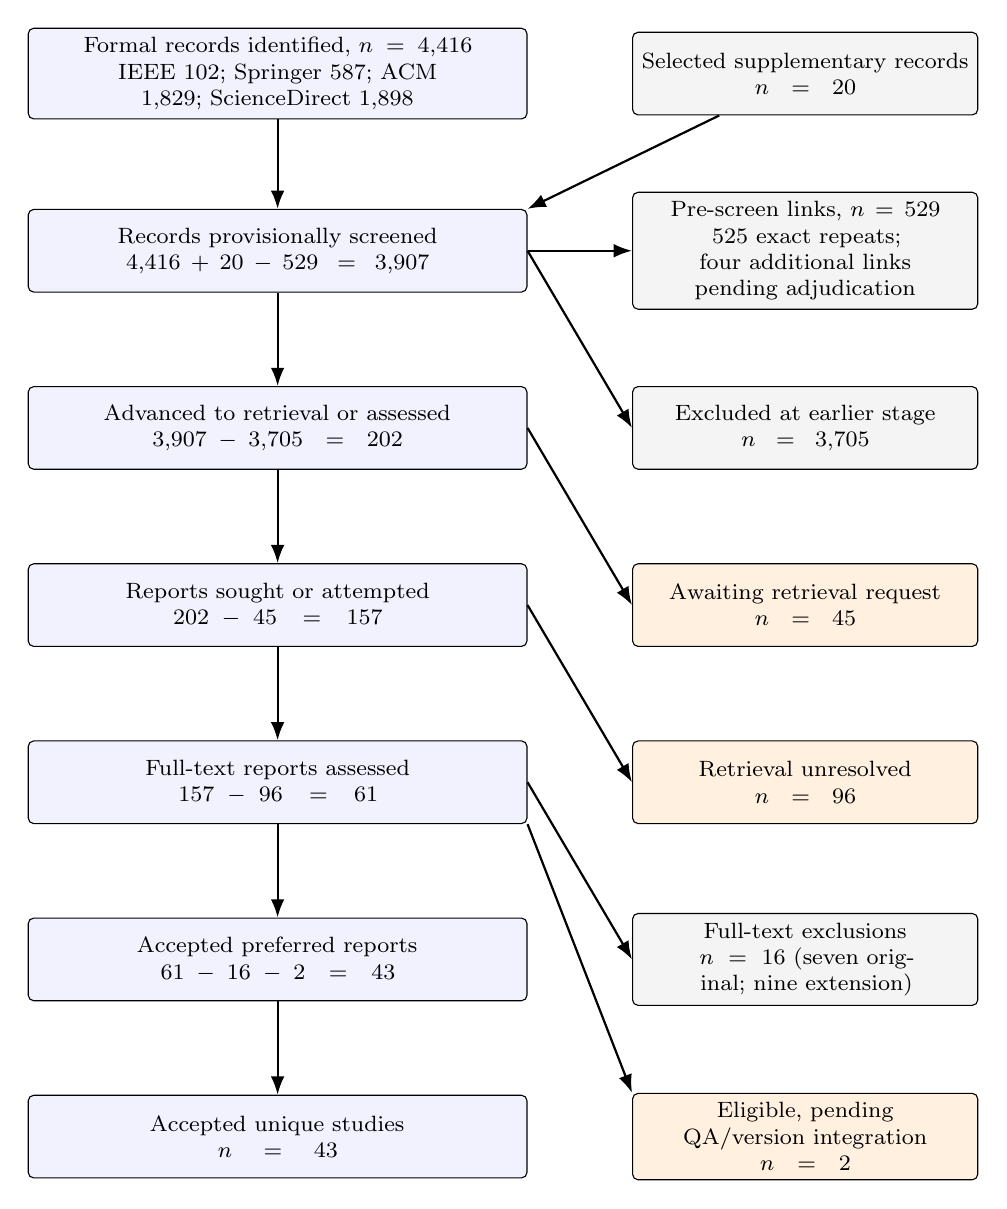
\begin{tikzpicture}[>=Latex, every node/.style={font=\footnotesize},
  main/.style={draw,rounded corners=2pt,align=center,text width=6.1cm,minimum height=1.05cm,fill=blue!5},
  side/.style={draw,rounded corners=2pt,align=center,text width=4.15cm,minimum height=1.05cm,fill=gray!9},
  open/.style={draw,rounded corners=2pt,align=center,text width=4.15cm,minimum height=1.05cm,fill=orange!12},
  line/.style={-Latex,thick}]
\node[main] (identified) at (0,0) {Formal records identified, $n=4{,}416$\\IEEE 102; Springer 587; ACM 1,829; ScienceDirect 1,898};
\node[side] (supp) at (6.7,0) {Selected supplementary records\\$n=20$};
\node[main] (screened) at (0,-2.25) {Records provisionally screened\\$4{,}416+20-529=3{,}907$};
\node[side] (dups) at (6.7,-2.25) {Pre-screen links, $n=529$\\525 exact repeats; four additional links pending adjudication};
\node[main] (advanced) at (0,-4.5) {Advanced to retrieval or assessed\\$3{,}907-3{,}705=202$};
\node[side] (early) at (6.7,-4.5) {Excluded at earlier stage\\$n=3{,}705$};
\node[main] (sought) at (0,-6.75) {Reports sought or attempted\\$202-45=157$};
\node[open] (unsought) at (6.7,-6.75) {Awaiting retrieval request\\$n=45$};
\node[main] (assessed) at (0,-9) {Full-text reports assessed\\$157-96=61$};
\node[open] (unavailable) at (6.7,-9) {Retrieval unresolved\\$n=96$};
\node[main] (accepted) at (0,-11.25) {Accepted preferred reports\\$61-16-2=43$};
\node[side] (excluded) at (6.7,-11.25) {Full-text exclusions\\$n=16$ (seven original; nine extension)};
\node[main] (studies) at (0,-13.5) {Accepted unique studies\\$n=43$};
\node[open] (integration) at (6.7,-13.5) {Eligible, pending QA/version integration\\$n=2$};
\draw[line] (identified) -- (screened);
\draw[line] (supp) -- (screened.north east);
\draw[line] (screened.east) -- (dups.west);
\draw[line] (screened) -- (advanced);
\draw[line] (screened.east) -- (early.west);
\draw[line] (advanced) -- (sought);
\draw[line] (advanced.east) -- (unsought.west);
\draw[line] (sought) -- (assessed);
\draw[line] (sought.east) -- (unavailable.west);
\draw[line] (assessed) -- (accepted);
\draw[line] (assessed.east) -- (excluded.west);
\draw[line] (assessed.south east) -- (integration.north west);
\draw[line] (accepted) -- (studies);
\end{tikzpicture}
\caption{Interim PRISMA 2020 stage map for the four captured database sources and selected supplementary records, 17 October 2026. The 529 pre-screen links include four Step 5 links awaiting canonical record/report adjudication; the 3,907 screening count is provisional. The 45 unsought reports and 96 unresolved retrieval cases are open, and two eligible reports await formal QA and version integration. Counts represent parsed occurrences, not verified search coverage; publisher hit/export discrepancies remain open. Source arithmetic and limitations: \texttt{interim\_four\_source\_prisma.json}.}
\label{fig:prisma-interim-four-source}
\end{figure}
\clearpage


\section{Historical 11 October screening checkpoint and reconciliation}
Every formal occurrence receives a record ID. Exact DOI/URL and normalized-title checks link duplicate occurrences without deleting provenance. Bibliographic report IDs identify candidate reports; study IDs identify accepted underlying studies. The REEF journal extension is selected for GA-S001; its less complete conference report is a linked E8 companion and adds no study.
\begin{longtable}{P{0.7\linewidth}r}\toprule Checkpoint quantity & Count\\\midrule\endhead
Formal query occurrences & 689\\
Duplicate occurrences & 10\\
Unique formal records & 679\\
Selected supplementary records & 20\\
Excluded before full text & 575\\
Full texts assessed & 28\\
Full-text exclusions & 7\\
Accepted unique studies & 21\\
Pending / not retrieved & 96\\
\bottomrule\end{longtable}
The reconciled captured subset is: 689-10+20=699 records; 699 equals pre-full-text exclusions plus assessed reports plus pending records. Assessed reports equal included reports plus full-text exclusions. The later ACM/ScienceDirect occurrence population is outside these 11 October arithmetic identities. This historical checkpoint remains separate from Figure~\ref{fig:prisma-interim-four-source}. Reports sought include pending retrieval attempts, but complete formal-database retrieval and final study-version resolution remain open.

\begin{figure}[p]
\centering
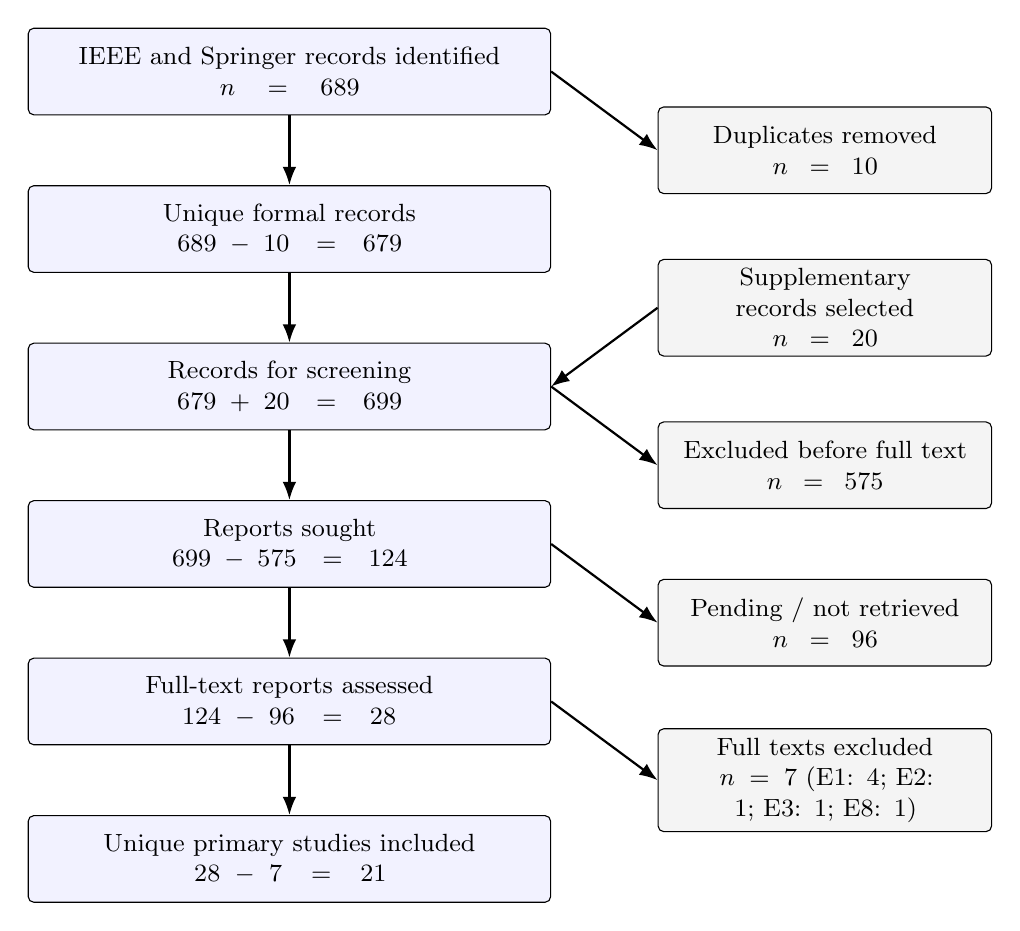
\begin{tikzpicture}[>=Latex, every node/.style={font=\small}, main/.style={draw,rounded corners=2pt,align=center,text width=6.4cm,minimum height=1.1cm,fill=blue!5}, side/.style={draw,rounded corners=2pt,align=center,text width=4.0cm,minimum height=1.1cm,fill=gray!9}, line/.style={-Latex,thick}]
\node[main] (id) at (0,0) {IEEE and Springer records identified\\$n=689$};
\node[main] (unique) at (0,-2) {Unique formal records\\$689-10=679$};
\node[side] (duplicate) at (6.8,-1) {Duplicates removed\\$n=10$};
\node[side] (supplementary) at (6.8,-3) {Supplementary records selected\\$n=20$};
\node[main] (screened) at (0,-4) {Records for screening\\$679+20=699$};
\node[main] (sought) at (0,-6) {Reports sought\\$699-575=124$};
\node[side] (early) at (6.8,-5) {Excluded before full text\\$n=575$};
\node[main] (assessed) at (0,-8) {Full-text reports assessed\\$124-96=28$};
\node[side] (unavailable) at (6.8,-7) {Pending / not retrieved\\$n=96$};
\node[main] (included) at (0,-10) {Unique primary studies included\\$28-7=21$};
\node[side] (excluded) at (6.8,-9) {Full texts excluded\\$n=7$ (E1: 4; E2: 1; E3: 1; E8: 1)};
\draw[line] (id) -- (unique);
\draw[line] (id.east) -- (duplicate.west);
\draw[line] (unique) -- (screened);
\draw[line] (supplementary.west) -- (screened.east);
\draw[line] (screened) -- (sought);
\draw[line] (screened.east) -- (early.west);
\draw[line] (sought) -- (assessed);
\draw[line] (sought.east) -- (unavailable.west);
\draw[line] (assessed) -- (included);
\draw[line] (assessed.east) -- (excluded.west);
\end{tikzpicture}
\caption{Interim PRISMA 2020 stage mapping for the reconciled 11 October captured subset. The later 3,727 ACM/ScienceDirect occurrences are outside this flow. E1--E8 reason definitions and report-level decisions are in \texttt{rejected.csv}. This is not the completed four-database flow.}
\label{fig:prisma-checkpoint}
\end{figure}
\clearpage

Title decisions are first-pass relevance judgments, explicitly labelled as title stage. Abstract decisions cite publisher scope; full-text decisions identify a section or experiment. Training and inference are not interchangeable: PipeSwitch and SIRIUS are retained for explicit inference outcomes, whereas TGS is rejected for training-only evidence. The Fermilab paper was retained after its multi-model slice experiment was inspected, rather than merely because it mentioned MIG. DIPPM was rejected because profile prediction alone does not test concurrent tenant sharing.

Full-text rejection examples include DIPPM (no concurrent tenant comparison), the accelerator-pool vRAN simulation and the low-latency FEC offloading paper (no inference evidence), DRMaestro's Rodinia workload evaluation (no serving inference), CalcGraph (assigned GPU partitioning left to future work), and the mediated-device passthrough benchmark (HPC applications without inference). The complete reasons and stages are in \texttt{rejected.csv}. Pending files have no fabricated technical results or QA scores.

\section{Batch 1: full-text decisions and batch-1 accepted checkpoint}\label{sec:batch1}

Ten user-supplied full-report conversions were received and assessed on 17 October 2026 by AI-CODEX. All ten satisfy the adopted eligibility rules and add distinct studies, GA-S022--GA-S031. At this batch checkpoint, the accepted evidence set contained \textbf{31 unique studies (21+10)}. This is an accepted-set update, not a claim that four-database screening or the final PRISMA flow is complete. Pantheon and Jormungandr retain their earlier eligible-pending-integration status and are outside the 31.

The supplied 76-record deduplicated download queue recorded ten at the batch-1 checkpoint received and assessed reports and 66 then awaiting assessment. The extension full-text register contains twelve assessed reports: the ten accepted here and the two earlier preliminary assessments. Received files are not re-requested. Occurrences, reports, and unique studies remain separate counting units.

\subsection{Eligibility, publication window and report identity}

The first-page DOI/title matches were checked against the occurrence ledger, the prior 21-study set, and the other reports in this batch. No duplicate study was identified. MIGER, BOER and MMK describe distinct designs and evaluations despite related mechanisms and citations. EnerTune cites an earlier workshop precursor; it is a version lead, not a second included study. All four 2026 reports have printed publication or conference dates before 11 October: MMK (July), MIGServe and AdMix (28 September--1 October), and EnerTune (29 September--2 October). Exact online dates remain distinct from event/issue dates. Deft retains export publication year 2024 and printed WoC 2023 event/reference dates; this discrepancy does not change eligibility.

Deft and AdMix are full original workshop proceedings reports with implemented evaluations, not poster abstracts. Their limited experiment breadth is reflected in appraisal and transfer caveats. Mixed inference/training studies qualify only for their explicit inference-specific local sharing evidence. Multi-GPU aggregate improvements remain separately labelled.

\begin{longtable}{P{0.14\linewidth}P{0.22\linewidth}P{0.44\linewidth}r}

\toprule Study & Report & Eligible evidence stratum & QA\\\midrule\endhead

GA-S022 & miger \cite{miger} & MIG partitions with per-partition MPS online/offline co-location, local partition planner and fragmentation control & 8\\

GA-S023 & deft \cite{deft} & Deft: adaptive CUDA synchronization frequency controlling kernel queues and priority preemption; API interposition prototype & 7\\

GA-S024 & fastgshare \cite{fastgshare} & FaST-GShare: MPS spatial shares plus CUDA interception/token-based temporal quotas; CUDA IPC model sharing & 7.5\\

GA-S025 & split \cite{split} & SPLIT: genetic offline model-block splitting with token-based greedy temporal preemption & 8.5\\

GA-S026 & migserve \cite{migserve} & MIGServe: buddy-aware MIG placement, proactive pair migration and temperature-guided eviction & 8\\

GA-S027 & mmk \cite{mmk} & MMK: MIG, elastic MPS oversubscription and CUDA-intercepted kernel-priority scheduling & 8\\

GA-S028 & boer \cite{boer} & BOER: MIG model grouping with Bayesian-optimized MPS configurations inside partitions & 8.5\\

GA-S029 & admix \cite{admix} & AdMix: adaptive MPS active-thread caps, lightweight LLM estimator and best-effort pause/full-access controls & 8.5\\

GA-S030 & sgdrc \cite{sgdrc} & SGDRC: CUDA/TVM runtime with software VRAM-channel coloring, bimodal tensors and tidal SM masks & 8.5\\

GA-S031 & enertune \cite{enertune} & EnerTune: MIG allocation with joint frequency/batch selection, colocation-power model and runtime tuner; separate MPS portability experiments & 9\\

\bottomrule\end{longtable}

\subsection{Bounded extraction and contradictory evidence}

\paragraph{GA-S022 miger.} Section 3.1/Fig. 2 directly compares local MPS 57/29/14 percent and MIG 4g/2g/1g allocations. Section 5.2/Fig. 8 reports testbed mean JCT 46.6\% below MuxFlow and 36\% below MISO; these are job/cluster outcomes, not inference p99 gains. Fig. 9 notes slower small jobs under MIGER. Includes mixed training/inference and multi-GPU optimization; retain only explicitly local sharing and inference-QoS evidence for assigned comparison. Abstract and introduction swap comparator order for the two JCT percentages; use section 5.2 mapping. No chart coordinates reconstructed or universal p99 claim. \textit{Source:} Printed pp. 505-506, 510-511; sections 3.1-3.3, 5.1-5.4; Tables 1-3; Figs. 2, 4, 8-11; N00001.md lines 119-229, 478-662.

\paragraph{GA-S023 deft.} Sections 3.2 and 5 show optimal synchronization depends on batch and image size; the fixed strategy can impose much larger preempting-job JCT inflation after a workload change. Section 5.2 reports Deft switches to synchronizing every kernel for batch 30; earlier batch-1 case uses every 500 kernels. Table 2 cells are interleaved, so no exact violation-rate row is imported. Preliminary six-page workshop evaluation with two principal models and one A40. Exhaustive pair profiling does not scale; no cluster/generative-model implementation claimed (section 6). Keep export year 2024 and printed conference/reference year 2023 separately; both inside window. \textit{Source:} Printed pp. 15-17; sections 3.2, 4.2, 5.1-5.3 and 6; Table 2 and Fig. 4 discussed in prose; N00005.md lines 250-468.

\paragraph{GA-S024 fastgshare.} Local section 5.3 states eight RNNT pods at 12\% SM shares reach about 40 req/s with tail latency below 500 ms, versus one racing pod about 12 req/s and above 1250 ms. The local ResNet/RNNT comparison in Fig. 9 reports removing their observed interference with 24\% shares. No unlabelled tail value is relabelled p99. Model-specific/proportional share effects, IPC memory trust and batching limit transfer. Prose fractional-gain notation is ambiguous (3.15x with raw 296.8/71.37), so no such multiplier imported. Supplied plot coordinates/percentile identity and repetitions not reconstructed. \textit{Source:} Printed pp. 641-643; sections 4, 5.1-5.4; Figs. 8-10; N00015.md lines 523-735.

\paragraph{GA-S025 split.} Section 5.5 reports violation rate below 10\% beyond alpha=4 versus 26\% under RT-A in the discussed comparison. For short requests, jitter reductions versus Clockwork/PREMA/RT-A are 55.3/46.8/68.9\% at low load and 56.0/50.3/69.3\% at high load. Jitter is block-execution standard deviation, not p99 latency. Section 6 reports split overhead and static-graph limits. One edge GPU and synthetic Poisson load; not a server-class GPU generalization. Temporal predictability sacrifices spatial parallelism; long-request stability can worsen. Table 3 split overhead and RNN limits qualify short-request improvements. \textit{Source:} Printed pp. 611-613; sections 5.1-5.5, 6; Tables 1-3; Figs. 6-7; N00040.md lines 451-629.

\paragraph{GA-S026 migserve.} Section 5.2 Azure: sustainable rate at 90\% SLO attainment is 9.84 RPS versus LA-Dyn 4.13 and Static 1.85. Arena approximately 10.99 versus 2.37 and 2.48 RPS. These are four-GPU server outcomes; local mechanism is MIG layout control, not a single-GPU throughput multiplier. Four-GPU evaluation and constructed layout-agnostic comparator; 90\% attainment is weaker than 99\% SLO targets used elsewhere. MIG hardware isolation is described, without adversarial/fault experiment. Source pixels and unreported repeats/versions are not reconstructed. \textit{Source:} Printed pp. 850-853; sections 4, 5.1-5.4; Fig. 9 and Figs. 11-13; N00831.md lines 519-780.

\paragraph{GA-S027 mmk.} Section 4.3/Fig. 9 reports mean JCT 28\% lower, makespan 32\% lower and normalized progress-rate STP 35\% higher than MIGER. These are mixed-job/testbed metrics, not per-request p99 latency. Section 4.5 reports 1.5\% MIG and 3.2\% MPS reconfiguration lifecycle overhead. Mixed inference/training and two-GPU optimization; local priority scheduling is the transferable mechanism. Many figure labels contain NUL/glyph corruption, so numerical prose only. STP/JCT does not establish online tail-latency or fault containment. \textit{Source:} Article pp. 84:15-84:19; sections 4.1-4.5; Table 3; Figs. 9-12; N00839.md lines 789-1040.

\paragraph{GA-S028 boer.} Local section 2.4/Fig. 3 observes ParvaGPU can underperform MIG-only serving for larger BERT/ResNet50 while helping lightweight MobileNet. Section 5.2/Fig. 8 gives eight-GPU QoS-preserved throughput mean 34.61\% above ParvaGPU; 56.8/62.49/34.63/44.83\% above MIG-serving/gpulet/USHER/PARIS. Keep local qualitative counterexample separate from fleet improvements. Bayesian exploration cost and instance interference qualify hybrid gains. Baseline reductions (MIG-serving fast/USHER IR only) and multi-GPU request fan-out constrain comparison. Same senior author as MIGER, but different inference-only system and experiments; not a same-study report extension identified in supplied text. \textit{Source:} Printed pp. 521, 526-528; sections 2.4, 4.6, 5.1-5.4; Tables 2-3; Figs. 3, 8, 10; N00844.md lines 200-265, 700-890.

\paragraph{GA-S029 admix.} Section 4.2 reports average best-effort throughput 1.58x Static MPS with local LLaMA-7B (TP1) and 3.9x with Qwen-14B (TP2), keeping strata distinct. AdMix still increases mean TTFT/TPOT versus LLM-only; on Qwen its mean latency increases exceed Static MPS. More throughput is not zero interference. Full six-page original workshop report; one/two-GPU workload strata and tuned-on-test-trace static reference limit transfer. Estimates of average latency do not establish p99. No testbed code rerun or security/fault experiment inferred. \textit{Source:} Printed pp. 3-5; sections 3 and 4.1-4.2; Table 1; Figs. 5-6; N00872.md lines 270-453.

\paragraph{GA-S030 sgdrc.} Section 9.3: versus Orion, P40 overall throughput up to 1.47x and BE up to 2.36x; A2000 up to 1.32x and 1.79x, respectively. Mean SLO attainment 99.0\% across evaluated settings. Section 10 explicitly states shared-context GPU runtime errors are not isolated. Software coloring is not a proven security boundary. MIG integration is future work; not benchmarked on A100/H100. Reverse-engineering/calibration and TVM compatibility matter; do not treat throughput maxima as averages or infer a P40 MPS result. \textit{Source:} Printed pp. 276-277; sections 9.2-9.3, 10; Table 3 and Fig. 18; N00904.md lines 863-965.

\paragraph{GA-S031 enertune.} Section 2.1/Fig. 2: co-location choice can increase energy; SDXL plus MobileNetV3 example uses 13\% less energy versus no sharing despite 1.14x latency. Section 7.1/Fig. 9: 16-GPU testbed energy reduced by factors 1.4-2.3 and power by 1.3-2.6 versus baselines while meeting SLOs; fleet results are not local per-GPU savings. Joint power/energy objectives select different allocations. Local model-pair evidence must stay distinct from fleet savings and from frequency-only effects. Source chart pixels not available; experiments/code not rerun; missing warm-up and independent-run uncertainty not assumed. \textit{Source:} Printed pp. 66-67, 73-75; sections 2.1-2.2, 6, 7.1-7.2; Figs. 2, 9; N00946.md lines 140-249, 798-995.

\subsection{Quality, isolation and sensitivity}

The ten batch scores total 81.5/100. At the 31-study batch-1 checkpoint, the total is 255.5/310 (mean 8.24); 25 high, 6 moderate and 0 low. The original Q1--Q10 rubric is unchanged. Each new item score has a rationale and source anchor in \path{batch1_quality.csv}; \path{current_quality.csv} combines the historical and batch registers. The evidence cards included 31 studies at this checkpoint; batch 2 later updates the combined cards.

Excluding moderate-QA reports removes Deft and FaST-GShare from this batch as well as the four moderate reports in the earlier set. This weakens adaptive synchronization and serverless quota evidence; it does not establish that all remaining studies have comparable or complete measurement controls. No numerical effect is pooled across studies.

SGDRC explicitly cannot contain co-located GPU runtime faults in its shared context (section 10). MIG-based partition descriptions do not establish adversarial security or fault-injection results. AdMix and EnerTune show why higher throughput or utilization is insufficient: protected-service latency and energy can worsen under particular sharing configurations. These are conditional trade-offs, not universal rankings.

\subsection{Evidence and remaining work}

The historical 11 October registers and flow remain available unchanged. Extension decisions are authoritative in \path{new_fulltext_assessments.csv}, supported by \path{batch1_review_assessments.json}, per-item QA, extraction and SHA-256 receipts. The combined accepted views are \path{current_accepted.csv}, \path{current_extraction.csv}, \path{current_quality.csv} and \path{current_included_studies.json}. The workbook Included and Quality tabs showed 31 studies at this checkpoint; its Summary tab is explicitly historical and Current shows the later accepted set. The bibliography contained 31 preferred reports at this checkpoint.

\pending{Complete the remaining retrieval/eligibility records, reconcile the supplied Step 3--5 decisions and duplicate/version links, integrate or resolve the two earlier extension assessments, and derive a complete four-database PRISMA flow. The 66 entries remaining at this checkpoint are candidate reports, not guaranteed additions. No unavailable chart data, reviewer consensus, or screening outcome is invented.}

\section{Batch 2: full-text reassessment}\label{sec:batch2}

Eleven further user-supplied full-report conversions from the deduplicated queue were assessed on 17 October 2026 by the same single AI reviewer. Three add unique studies GA-S032--GA-S034; eight are excluded with principal full-text reasons. Prior rule-assisted title/abstract exclusions were reconsidered when the full texts arrived. The accepted set is now \textbf{34 unique studies (21 historical + 10 batch 1 + 3 batch 2)}; this does not complete merged database screening or PRISMA accounting.

The 76-entry download queue has 21 received reports (13 accepted, eight excluded) and 55 unassessed entries. The extension full-text ledger has 23 assessed reports, including two older eligible-pending-integration reports outside the 34. Source hashes, reasons and anchors are retained without committing paper bodies.

\subsection{Decisions and evidential bounds}

\begin{longtable}{P{0.16\linewidth}P{0.22\linewidth}P{0.52\linewidth}}\toprule Record & Decision & Primary reason or direct evidence\\\midrule\endhead

GA-N00920 & Accept GA-S032 \cite{fluidfaas} & Include: original HPDC full paper evaluates concurrent inference functions with local MIG partitioning and request SLO outcomes; separate server-level from local mechanism claims.\\

GA-N01085 & Accept GA-S033 \cite{bless} & Include: original EuroSys full paper explicitly evaluates co-located inference instances with an implemented single-A100 temporal/MPS hybrid.\\

GA-N01096 & Accept GA-S034 \cite{interference_deeper} & Include as direct interference/isolation evidence: real single-GPU LLM inference is concurrently run with a distinct synthetic process/kernel under streams and Green Context SM partition; a mixed co-tenant experiment is explicitly bounded, with no claim of two production inference services.\\

GA-N00002 & Exclude E2 & Cricket/unikernel CUDA remoting is evaluated with microbenchmarks and proxy applications across two nodes, without a concurrent inference-tenant GPU comparison. The JetsonInference library appears in related work, not the evaluated setting.\\

GA-N00004 & Exclude E1 & AWS Lambda/rCUDA case study compares CPU, native GPU and remote GPU for a single GPU-BLAST processing path; AI inference is motivation, without measured inference-serving outcomes for concurrent tenants.\\

GA-N00055 & Exclude E4 & nvshare's measured co-located TensorFlow ResNet152v2 applications train models; the authors explicitly select training-only evaluation although inference is mentioned as background.\\

GA-N00088 & Exclude E1 & GPUPool evaluates throughput-oriented long jobs and simulated kernel pairs; inference appears as a motivating workload class/reference, without an inference-specific measured serving outcome.\\

GA-N00102 & Exclude E2 & Guardian's multi-application spatial-sharing comparison uses epoch-based training/co-run workloads (Table 2, Fig. 6); inference phases are tested standalone for overhead (Fig. 7b). There is no evaluated concurrent inference-serving arrangement under the adopted criterion.\\

GA-N01195 & Exclude E2 & ReFINE evaluates synthetic priority kernel pairs in Accel-Sim architectural simulation rather than a measured concurrent inference arrangement on one physical GPU; inference serving is an illustrative motivation.\\

GA-N01866 & Exclude E1 & Edge-device rCUDA evaluation runs the Fuzzy Minimals clustering algorithm across remote node/GPU settings; no inference-serving workload or outcome is evaluated.\\

GA-N01945 & Exclude E1 & MIG scheduling and reconfiguration evaluates Rodinia/Altis benchmarks and synthetic task queues for makespan; inference latency is that of the DRL scheduler itself, not a model-serving tenant outcome.\\

\bottomrule\end{longtable}

\paragraph{GA-S032 fluidfaas.} Section 7.1/Fig. 9 reports FluidFaaS SLO hit-rate improvement of 90\% for medium and 61\% for heavy workload mixes over the compared systems; the abstract reports 25–75\% throughput increases across workloads. These are system-level results, not a measured per-GPU utilization effect. Pipeline, placement and MIG allocation contribute jointly; comparisons with a non-pipelined baseline cannot isolate the benefit of MIG partitioning alone. No adversarial security or fault-injection evidence is inferred from MIG descriptions. \textit{Anchor:} N00920.md abstract, sections 3, 6, 7.1; Tables 2, 5–6; Figs. 9 and 12.

\paragraph{GA-S033 bless.} The introduction and evaluation report mean latency reductions of 39.1\% for two BERT inference instances and 41.2\% for four, under the paper's compared GPU-sharing systems. Other reported aggregate gains are not recast as p99 or universal speedups. Quota, model pairing and GPU generation condition results. The conversion has damaged column/table layout, so no unlabeled plotted coordinates or precise tail-percentile gains were recovered. \textit{Anchor:} N01085.md intro, sections 4, 6.1–6; Fig. 1 and BERT co-location result prose.

\paragraph{GA-S034 interference\_deeper.} H100 Llama decode P90 time between tokens rises from 7.53 to 16.56 ms under a sleep co-tenant in section 4.2 (batch 1, 1,000-token prompt). Table 1's Green Context experiment isolates SM sets (64/68) but reports P90 TBT as high as 18.38 ms under copy-kernel memory pressure; its alone baseline is 14.2 ms on the whole GPU, so partition cost and interference cannot be collapsed into one effect. Synthetic co-tenants and short decode traces quantify resource contention; the paper proposes a future scheduler but does not implement an end-to-end serving controller. Green Context SM partition does not partition L2 or external memory bandwidth. Table 1 conversion is interleaved; only prose and clearly attributable values are used. \textit{Anchor:} N01096.md sections 3–5, especially 4.1–4.4; Fig. 2 and Table 1.

\subsection{Appraisal and remaining reconciliation}

The three new studies score 24/30; the combined 34 score 279.5/340, with 28 high, 6 moderate, and 0 low. The same Q1--Q10 rubric applies only to included studies. Source-specific Q-item rationales and limitations are in \path{batch2_quality.csv} and \path{batch2_extraction.csv}.

The SoCC paper prints a November 2025 event date although the export lists 2026; both lie within the cutoff. It measures synthetic kernel co-tenants alongside LLM inference, not two production inference services. Guardian shows co-located training and standalone inference only; it therefore fails the adopted concurrent inference criterion despite useful memory-safety context.

\pending{Resolve 55 remaining queue entries, the two older eligible-pending-integration reports, report-version and occurrence links, and the four-database PRISMA flow. Excluded batch-2 reports are assessed full texts, not additions to the historical Flow A seven full-text exclusions.}

\section{Batch 3: full-text review}\label{sec:batch3}

Ten further user-supplied full-report conversions were assessed by one AI reviewer on 17 October 2026. Nine add unique studies GA-S035--GA-S043; one is excluded. The accepted set is now \textbf{43 unique studies (21 historical + 10 batch 1 + 3 batch 2 + 9 batch 3)}. This is not a reconciled merged-database PRISMA inclusion count. The 76-entry queue has 31 assessed reports and 45 unassessed entries. Two older eligible-pending-integration reports remain outside the 43.

\begin{longtable}{P{0.16\linewidth}P{0.22\linewidth}P{0.52\linewidth}}\toprule Record & Decision & Reason or bounded finding\\\midrule\endhead

GA-N00027 & Accept GA-S035 \cite{edge_sky} & Include: original journal evaluation has concurrent inference on local edge GPU, with heterogeneous results interpreted separately.\\

GA-N00046 & Accept GA-S036 \cite{miriam} & Include: original full conference paper measures concurrent inference and critical-task latency on edge GPUs.\\

GA-N00048 & Accept GA-S037 \cite{elasticroom} & Include: original full conference evaluation of concurrent tenants on a shared GPU with inference latency/goodput outcomes.\\

GA-N00049 & Accept GA-S038 \cite{switchflow} & Include: section 5.4 directly evaluates two inference jobs sharing one GPU; mixed training experiments are qualified separately.\\

GA-N00059 & Accept GA-S039 \cite{itif} & Include: original full proceedings evaluation of simultaneous transformer inference tenants sharing GPU resources.\\

GA-N00063 & Accept GA-S040 \cite{protean} & Include with scope qualification: original paper implements local MIG/MPS inference sharing and evaluates concurrent inference, while synthesis separates system-level outcomes.\\

GA-N00068 & Accept GA-S041 \cite{wattwiser} & Include with scope qualification: measured local shared-GPU inference pairs occur on one server; aggregate energy is contextual only.\\

GA-N00070 & Accept GA-S042 \cite{deinfer} & Include: original full paper tests concurrent inference and local MPS spatial resource allocations.\\

GA-N00073 & Accept GA-S043 \cite{esg} & Include with scope qualification: original full paper evaluates local GPU sharing of inference functions embedded in a serverless workflow.\\

GA-N00018 & Exclude E4 & IADeep evaluates co-located iterative deep-learning training jobs and training throughput. Inference is not an evaluated concurrent tenant workload under the adopted inference criterion.\\

\bottomrule\end{longtable}

\paragraph{GA-S035 edge\_sky.} Abstract and multi-tenancy evaluation report inference throughput gains under concurrent execution; do not attribute heterogeneous placement gains solely to GPU sharing. Edge GPU, CPU and TPU contributions are coupled; throughput is not latency predictability or security isolation. \textit{Anchor:} N00027.md abstract; multi-tenancy and performance evaluation sections, figures on CME and DMP.

\paragraph{GA-S036 miriam.} Abstract reports up to 92\% throughput improvement while critical tasks incur less than 10\% latency overhead in its evaluated scenarios. Edge elastic-kernel scheduling is transferable temporal/spatial evidence, not a direct MIG/MPS comparison. \textit{Anchor:} N00046.md abstract; sections on kernel coordination and evaluation.

\paragraph{GA-S037 elasticroom.} The evaluated engine balances request goodput, throughput and latency under co-located inference; comparison is engine-level. Compiler and priority scheduling effects cannot be isolated as pure partition effects; plotted numbers were not transcribed. \textit{Anchor:} N00048.md abstract; section 6.2 evaluation and Fig. 1.

\paragraph{GA-S038 switchflow.} Section 5.4/Fig. 10 reports interleaved execution gains among inference jobs of up to 30\% versus session-based time slicing in tested pairings. The 19.05x p95 inference latency example in Fig. 6 uses a training co-tenant and is not evidence for two inference tenants. \textit{Anchor:} N00049.md sections 5.1, 5.2.1 and 5.4; Figs. 6 and 10.

\paragraph{GA-S039 itif.} Abstract reports up to 2.40x performance versus baselines for evaluated shared-backbone transformer inference. Shared backbone changes model computation; speedup cannot be assigned to GPU scheduling alone or generalized to unrelated models. \textit{Anchor:} N00059.md abstract; design and experiment sections including four-tenant setup.

\paragraph{GA-S040 protean.} The evaluation reports SLO compliance and cost effects of orchestration under trace-driven inference; no per-GPU improvement is extracted from system-level totals. Multiple GPUs and global scheduling contribute jointly; local mechanism claims cannot be isolated without matched per-device comparisons. \textit{Anchor:} N00063.md abstract, sections on MIG/MPS design and evaluation of 22 workloads.

\paragraph{GA-S041 wattwiser.} Section 4/Fig. 3 shows model tail latency relative to SLO while requests consolidate onto shared GPUs; power savings are whole-server effects. The four-GPU power outcome cannot estimate per-GPU partition efficiency; MI50 setup is not a MIG evaluation. \textit{Anchor:} N00068.md sections 4.1–4.2 and Fig. 3.

\paragraph{GA-S042 deinfer.} Section 5 evaluates prediction accuracy and allocation for concurrent inference with MPS; its Fig. 2 shows that MPS spatial limits do not eliminate shared-resource latency interference. Two GPUs are present in testbed; claims here concern within-device workloads, not a two-device pooled speedup. \textit{Anchor:} N00070.md sections 2.2 and 5.1–5.2; Fig. 2, Table 1 and testbed table.

\paragraph{GA-S043 esg.} Abstract reports 61–80\% SLO hit-rate improvement and 47–187\% cost savings over prior systems for evaluated workflows. Figures are workflow/system results influenced by batching and scheduler search, not isolated effects of local GPU sharing. \textit{Anchor:} N00073.md abstract, sections 3 and 5; evaluation setup and end-to-end comparison.

\pending{The batch-3 reports extend the assessed evidence, not the historical Flow A boxes. Reconcile the remaining 45 queue entries, two older eligible reports, duplicate/version links, database searches and the combined PRISMA flow.}


\section{Historical 21-study accepted checkpoint}
The following studies are accepted for this intermediate evidence set. \pending{The study list, preferred reports and QA totals may change after the new search population is screened and version links are settled.} KRISP is a scope-boundary inclusion under protocol 7.2 because it evaluates local spatial resource control and inference workers; its emulated AMD feature and non-NVIDIA baseline are explicitly isolated in synthesis. No vendor document or preprint-only unpublished work counts toward this table.
\begin{longtable}{P{0.15\linewidth}P{0.25\linewidth}P{0.4\linewidth}r}
\toprule Study & Report/year & Mechanism / scope & QA\\\midrule\endhead
GA-S001 & REEF 2025 \cite{reef} & Reset-based temporal preemption + dynamic kernel padding; NVIDIA binary instrumentation & 8.5\\
GA-S002 & GPULET 2022 \cite{gpulet} & MPS + temporal & 8.5\\
GA-S003 & PIPESWITCH 2020 \cite{pipeswitch} & Temporal context switching & 9.0\\
GA-S004 & CLOCKWORK 2020 \cite{clockwork} & Temporal exclusive scheduling & 8.5\\
GA-S005 & TORPOR 2025 \cite{torpor} & API remoting + temporal swapping & 8.5\\
GA-S006 & STREAMBOX 2024 \cite{streambox} & API/runtime sandbox virtualization & 8.0\\
GA-S007 & KRYPTON 2025 \cite{krypton} & Kernel API virtualization + hybrid & 9.0\\
GA-S008 & SIRIUS 2025 \cite{sirius} & Temporal + MPS memory handover & 8.5\\
GA-S009 & TALLY 2025 \cite{tally} & CUDA API interception + priority & 9.0\\
GA-S010 & PARVA 2024 \cite{parva} & MIG + MPS & 8.0\\
GA-S011 & ORION 2024 \cite{orion} & CUDA API interception + temporal & 9.0\\
GA-S012 & GSLICE 2020 \cite{gslice} & MPS adaptive provisioning & 9.0\\
GA-S013 & KRISP 2023 \cite{krisp} & Spatial partition/API control (AMD) & 8.0\\
GA-S014 & XSCHED 2025 \cite{xsched} & Temporal API interposition & 9.0\\
GA-S015 & PAELLA 2023 \cite{paella} & Temporal software scheduling + MPS comparison & 8.5\\
GA-S016 & GNNTRITON 2024 \cite{gnntriton} & MIG + concurrent model serving & 8.5\\
GA-S017 & VASTPIPE 2025 \cite{vastpipe} & MPS adaptive quotas; separate AMD CU-mask stratum & 6.5\\
GA-S018 & ARKGPU 2023 \cite{arkgpu} & CUDA API interception + NVML monitoring and admission throttling & 7.0\\
GA-S019 & DYNAP 2025 \cite{dynap} & MIG dynamic placement/reconfiguration with reconfiguration-last policy & 7.0\\
GA-S020 & IGNITER 2023 \cite{igniter} & MPS active-thread quotas + interference-aware batch/provisioning and shadow process & 8.5\\
GA-S021 & INFERFAIR 2024 \cite{inferfair} & Temporal SLO-aware scheduling + feedback goodput balancing; MPS comparator & 7.5\\
\bottomrule\end{longtable}
USENIX proceedings PDFs are official published copies. ACM/IEEE author or camera-ready copies are linked to verified proceedings metadata and do not become separate preprint studies. ParvaGPU's author manuscript is provisional for publisher-version comparison; its reported runtime-version anomaly remains flagged. The supplied REEF journal conversion establishes a more complete implementation/evaluation; it is now the preferred report for GA-S001. The conference report is retained as a linked companion. Accessible copies of Orion, GSLICE, KRISP, Tally and Paella avoid unnecessary institutional download requests.

\Needspace{16\baselineskip}\subsection{Source-anchored finding register}\begin{longtable}{P{0.18\linewidth}P{0.48\linewidth}P{0.24\linewidth}}\toprule Study & Bounded finding & Source location\\\midrule\endhead
GA-S001 \cite{reef} & GV100 PyTorch DISB-C: Orion p 99 normalized latency 1.17x vs Reef below 1.05x; normalized total throughput 0.97x vs 1.14x(Fig 29). TensorRT comparison trades throughput: mean 1.21x Triton vs 1.11x Reef(Fig 28). All ratios retain model-solo normalization; do not mix engines/AMD strata. & Article pp 1:23-1:24,1:31-1:34; sections 6.2,6.6,7; Figs 28-29; Markdown lines 1111-1180,1600-1820\\
GA-S002 \cite{gpulet} & Local gpulets support interference-aware provisioning; cluster throughput is a different outcome. & PDF p 10 Table 2/3; section 5; local profiling section 3\\
GA-S003 \cite{pipeswitch} & Fig 7: inference preemption latency reduced by up to 38.2ms. & PDF pp 11-13; sections 6-6.2; Fig 7\\
GA-S004 \cite{clockwork} & Fig 5 measures goodput satisfying SLO, rather than raw request throughput. & PDF p 10; section 6.1; Fig 5\\
GA-S005 \cite{torpor} & BERT Table 4: native 42ms, remote 43ms, PCIe swap 144ms, NVLink swap 45ms. & PDF pp 10-11; Table 4; sections 7.2-7.3\\
GA-S006 \cite{streambox} & Table 2 evaluates runtime sandbox workflows on shared GPUs. & PDF p 10 onward; section 9; Table 2\\
GA-S007 \cite{krypton} & Inference-specific sharing comparisons; section 2.2 tests fault propagation. & PDF p 10 Tables 1-2; section 5; section 2.2 Fig 3\\
GA-S008 \cite{sirius} & Inference p 99/SLO outcomes accompany training progress; separate TTFT/TBT LLM case. & Section 6.1 Fig 10; section 6.6\\
GA-S009 \cite{tally} & At 10\% idle time: normalized throughput Tally 1.19 vs TGS1.65. & PDF pp 9-11; sections 5-5.3; Fig 6\\
GA-S010 \cite{parva} & Fig 7 separates internal/external fragmentation; Fig 5 counts GPUs. & PDF p 8 onward; sectionIV; TableIV; Figs 5/7\\
GA-S011 \cite{orion} & Interference-aware scheduling compares inference latency and BE throughput. & PDF pp 8-9; sections 5.3-6.1; Tables 1/3\\
GA-S012 \cite{gslice} & GUE measures efficiency; shadow instance loading takes about 12s in Fig 15. & PDF pp 8-12; section 4; Table 3; Fig 15\\
GA-S013 \cite{krisp} & Kernel-wise right-sizing evaluates throughput and p 95 inference latency. & PDF pp 9-10; sectionsV-VI; TableIII\\
GA-S014 \cite{xsched} & Fig 15: relative p 99 1.53/1.51/1.07 respectively versus solo. & PDF pp 14-15; section 8 Case 3 Fig 15; section 9\\
GA-S015 \cite{paella} & p 99 latency and throughput under bursty model mixes; Fig 12 includes MPS. & PDF pp 9-12; section 7 Table 3/Figs 11-12; section 8\\
GA-S016 \cite{gnntriton} & Fig 10: thrashing after two models/20GB or five/40GB. & HTML Multi-model Scaling/Fig 10; Triton implementation; limitations\\
GA-S017 \cite{vastpipe} & A100 VGG16+GoogLeNet: throughput 2.7x no MPS and 1.5x default MPS; not a universal average or p 99 result. NLP/CV mean 2.43x no MPS, 1.45x default MPS. MI100 mean 1.89x no mask, 1.24x default mask. & Published pp 457-459; sections 6.7-6.9; Figs 14-16; uploaded Markdown lines 1150-1290\\
GA-S018 \cite{arkgpu} & Section 5.2 reports all 30 tested pairs satisfy the 2x-solo p 99 QoS target with ArkGPU. Low-contention pairs can lose about 5\% QPS from throttling. Four-GPU app-mix goodput gains 94.98\% vs k 8s-native and 38.65\% vs MPS are separate system-level results. & Published pp 313-319; sections 4.3,5.1-5.4; Table 3; Figs 14-21; Markdown lines 920-1360\\
GA-S019 \cite{dynap} & Single-A30 batch experiments: smaller partitions increase concurrency but can increase mean JCT; not online p 99 evidence. Fig 8 broader job set reports 39.03\% lower makespan vs StaCon,12.14\% vs MISO and 14.7\% higher normalized STP vs StaCon. Prediction-error sensitivity:15\% perturbation adds 8.09\% makespan. & PDF pp 11-16; sections 4.1-4.3.2; Table 2; Figs 8-13; Markdown lines 700-865\\
GA-S020 \cite{igniter} & Local four-model latency prediction error 1.53\%-5.02\%(Fig 13). Fig 14 deployment: iGniter 6 GPUs/0 SLO violations vs gpu-lets+8/3,FFD+5/10,GSLICE+6/3;25\% lower hourly instance cost vs gpu-lets+, not 25\% higher local utilization. Fig 17 shows an initial p 99 violation before shadow-process recovery. & Published pp 820-824; sections 4.2,5.1-5.4; Figs 13-18; Markdown lines 938-1245\\
GA-S021 \cite{inferfair} & Local Table 3 load 3:1:2: unfairness 1.05 vs Clockwork 1.50; SLO goodput 524.29 vs 457.24req/s. Other load ratios give smaller differences. Local unfairness is max/min model slowdown(Eq 2), not p 99 or security. Four-GPU MAF outcome kept separate. & Published pp 17-18; sections 5.1-5.4; Table 3; Eq 2; Markdown lines 718-899\\
\bottomrule\end{longtable}
\section{Review of six supplied full texts}
Five reports add unique studies: VastPipe, ArkGPU, Dyna-P, iGniter and InferFair. REEF's journal report explicitly extends OSDI2022 with a complete NVIDIA implementation, additional kernel handling and newer comparisons; the journal is preferred within GA-S001. Six previously pending reports are now assessed; the earlier conference report becomes a full-text E8 companion. There are 21 accepted studies,28 assessed reports including 7 full-text exclusions, and 96 pending access cases. Search occurrence and discovery counts are unchanged.

The source files are Markdown conversions. Two-column interleaving, missing plot pixels and damaged mathematical symbols prevent exact extraction of some equations, CDFs, error bars and configurations. Only readable labelled tables, captions and explicitly stated numeric results enter the register. Missing values are not interpolated. The receipt ledger records filenames and SHA-256 hashes; licensed source contents are not published.

Local GPU strata determine inclusion. VastPipe's NPU-cluster outcomes, ArkGPU's four-GPU goodput, Dyna-P's multi-GPU aggregates and cluster simulation, iGniter's fleet cost, and InferFair's four-GPU trace are distinguished from local results. ArkGPU qualifies through the explicit mixed inference/training exception; transfer is limited to priority inference protection. Dyna-P's job completion and makespan do not establish online p 99. InferFair's unfairness is a relative slowdown ratio and does not establish adversarial isolation.

Journal REEF's same-engine GV100 PyTorch comparison reports DISB-C p 99 below 1.05 times solo versus 1.17 for Orion, alongside separately normalized total throughput. Its TensorRT comparison also reports lower mean normalized throughput than Triton; preserving this counterexample prevents a universal superiority claim. iGniter's initial p 99 violation followed by shadow-process correction likewise qualifies any steady-state SLO statement. Source locations and QA rationales are recorded per report.

At the stricter QA threshold 8, VastPipe, ArkGPU, Dyna-P and InferFair are omitted; their mechanism-specific conclusions weaken. At the protocol low-quality threshold 6, none is omitted. This is a reporting-quality sensitivity, not a pooled causal result. The set now exceeds the protocol's 15--20-study target range; retain all eligible studies at this checkpoint and document any final narrowing transparently rather than removing evidence to fit a count.

\section{Quality appraisal and extraction controls}
\subsection{Section 13: item-level quality assessment}

The adopted ten-item rubric scores reporting and interpretability from 0 (absent), 0.5 (partial) or 1 (adequate), for a maximum of 10. Eligibility was assessed separately. The preferred peer-reviewed report of each accepted study is scored once; the earlier Reef conference version remains in the assessment history but does not add a study. The same single AI reviewer prepared all scores. No independent agreement statistic or experimental replication is claimed.

\begingroup\scriptsize\setlength{\tabcolsep}{3pt}

\begin{longtable}{P{0.14\linewidth}*{10}{>{\centering\arraybackslash}p{0.045\linewidth}}P{0.08\linewidth}P{0.10\linewidth}}

\toprule Study & Q1 & Q2 & Q3 & Q4 & Q5 & Q6 & Q7 & Q8 & Q9 & Q10 & /10 & Band\\\midrule\endhead

\texttt{GA-S001} & 1 & 1 & 0.5 & 1 & 1 & 1 & 0.5 & 0.5 & 1 & 1 & 8.5 & high\\

\texttt{GA-S002} & 1 & 1 & 1 & 1 & 0.5 & 1 & 0.5 & 1 & 0.5 & 1 & 8.5 & high\\

\texttt{GA-S003} & 1 & 1 & 0.5 & 1 & 1 & 1 & 1 & 1 & 0.5 & 1 & 9 & high\\

\texttt{GA-S004} & 1 & 1 & 0.5 & 1 & 0.5 & 1 & 0.5 & 1 & 1 & 1 & 8.5 & high\\

\texttt{GA-S005} & 1 & 1 & 0.5 & 1 & 1 & 1 & 0.5 & 1 & 0.5 & 1 & 8.5 & high\\

\texttt{GA-S006} & 1 & 1 & 0.5 & 1 & 0.5 & 1 & 0.5 & 1 & 0.5 & 1 & 8 & high\\

\texttt{GA-S007} & 1 & 1 & 1 & 1 & 0.5 & 1 & 0.5 & 1 & 1 & 1 & 9 & high\\

\texttt{GA-S008} & 1 & 1 & 0.5 & 1 & 0.5 & 1 & 1 & 1 & 0.5 & 1 & 8.5 & high\\

\texttt{GA-S009} & 1 & 1 & 0.5 & 1 & 1 & 1 & 0.5 & 1 & 1 & 1 & 9 & high\\

\texttt{GA-S010} & 1 & 1 & 0.5 & 1 & 0.5 & 1 & 0.5 & 1 & 0.5 & 1 & 8 & high\\

\texttt{GA-S011} & 1 & 1 & 0.5 & 1 & 0.5 & 1 & 1 & 1 & 1 & 1 & 9 & high\\

\texttt{GA-S012} & 1 & 1 & 0.5 & 1 & 1 & 1 & 1 & 1 & 0.5 & 1 & 9 & high\\

\texttt{GA-S013} & 1 & 1 & 1 & 1 & 0.5 & 1 & 0.5 & 1 & 0.5 & 0.5 & 8 & high\\

\texttt{GA-S014} & 1 & 1 & 0.5 & 1 & 1 & 1 & 0.5 & 1 & 1 & 1 & 9 & high\\

\texttt{GA-S015} & 1 & 1 & 0.5 & 1 & 0.5 & 1 & 0.5 & 1 & 1 & 1 & 8.5 & high\\

\texttt{GA-S016} & 1 & 1 & 0.5 & 1 & 0.5 & 1 & 0.5 & 1 & 1 & 1 & 8.5 & high\\

\texttt{GA-S017} & 1 & 1 & 0.5 & 1 & 0.5 & 1 & 0 & 0.5 & 0.5 & 0.5 & 6.5 & moderate\\

\texttt{GA-S018} & 1 & 1 & 1 & 1 & 0.5 & 1 & 0 & 0.5 & 0.5 & 0.5 & 7 & moderate\\

\texttt{GA-S019} & 1 & 1 & 0.5 & 1 & 0.5 & 1 & 0.5 & 0.5 & 0.5 & 0.5 & 7 & moderate\\

\texttt{GA-S020} & 1 & 1 & 0.5 & 1 & 0.5 & 1 & 1 & 0.5 & 1 & 1 & 8.5 & high\\

\texttt{GA-S021} & 1 & 1 & 0.5 & 1 & 0.5 & 1 & 0.5 & 1 & 0.5 & 0.5 & 7.5 & moderate\\

\texttt{GA-S022} & 1 & 1 & 0.5 & 1 & 0.5 & 1 & 0.5 & 1 & 1 & 0.5 & 8 & high\\

\texttt{GA-S023} & 1 & 1 & 0.5 & 1 & 0.5 & 1 & 0 & 0.5 & 1 & 0.5 & 7 & moderate\\

\texttt{GA-S024} & 1 & 1 & 0.5 & 1 & 0.5 & 0.5 & 0.5 & 1 & 0.5 & 1 & 7.5 & moderate\\

\texttt{GA-S025} & 1 & 1 & 0.5 & 1 & 0.5 & 1 & 0.5 & 1 & 1 & 1 & 8.5 & high\\

\texttt{GA-S026} & 1 & 1 & 0.5 & 1 & 0.5 & 1 & 0.5 & 1 & 0.5 & 1 & 8 & high\\

\texttt{GA-S027} & 1 & 1 & 1 & 1 & 0.5 & 1 & 0.5 & 0.5 & 0.5 & 1 & 8 & high\\

\texttt{GA-S028} & 1 & 1 & 0.5 & 1 & 0.5 & 1 & 0.5 & 1 & 1 & 1 & 8.5 & high\\

\texttt{GA-S029} & 1 & 1 & 0.5 & 1 & 0.5 & 1 & 0.5 & 1 & 1 & 1 & 8.5 & high\\

\texttt{GA-S030} & 1 & 1 & 0.5 & 1 & 0.5 & 1 & 0.5 & 1 & 1 & 1 & 8.5 & high\\

\texttt{GA-S031} & 1 & 1 & 1 & 1 & 0.5 & 1 & 0.5 & 1 & 1 & 1 & 9 & high\\

\texttt{GA-S032} & 1 & 1 & 0.5 & 1 & 0.5 & 1 & 0.5 & 1 & 1 & 0.5 & 8 & high\\

\texttt{GA-S033} & 1 & 1 & 1 & 1 & 0.5 & 1 & 0.5 & 1 & 0.5 & 0.5 & 8 & high\\

\texttt{GA-S034} & 1 & 1 & 1 & 0.5 & 0.5 & 1 & 0.5 & 1 & 1 & 0.5 & 8 & high\\

\texttt{GA-S035} & 1 & 1 & 0.5 & 0.5 & 0.5 & 1 & 0.5 & 1 & 0.5 & 0.5 & 7 & moderate\\

\texttt{GA-S036} & 1 & 1 & 0.5 & 1 & 0.5 & 1 & 0.5 & 1 & 1 & 0.5 & 8 & high\\

\texttt{GA-S037} & 1 & 1 & 0.5 & 1 & 1 & 1 & 0.5 & 1 & 0.5 & 0.5 & 8 & high\\

\texttt{GA-S038} & 1 & 1 & 1 & 1 & 1 & 1 & 0.5 & 1 & 1 & 1 & 9.5 & high\\

\texttt{GA-S039} & 1 & 1 & 0.5 & 1 & 0.5 & 1 & 0.5 & 1 & 1 & 0.5 & 8 & high\\

\texttt{GA-S040} & 1 & 1 & 1 & 1 & 0.5 & 1 & 0.5 & 1 & 1 & 0.5 & 8.5 & high\\

\texttt{GA-S041} & 1 & 1 & 1 & 1 & 1 & 1 & 0.5 & 1 & 1 & 1 & 9.5 & high\\

\texttt{GA-S042} & 1 & 1 & 1 & 1 & 0.5 & 1 & 0.5 & 1 & 1 & 1 & 9 & high\\

\texttt{GA-S043} & 1 & 1 & 0.5 & 1 & 0.5 & 1 & 0.5 & 1 & 1 & 0.5 & 8 & high\\

\bottomrule\end{longtable}\endgroup

The 43 preferred reports total 355 points (mean 8.26, range 6.5--9.5). There are 36 high (8--10), 7 moderate (6--7.5) and 0 low (below 6) scores. Their individual Q-item rationales, preferred-report IDs and source anchors are recorded in \path{current_quality.csv}; Appendix~\ref{app:cards} presents study-level evidence cards.

\begin{longtable}{P{0.11\linewidth}P{0.50\linewidth}rrr}

\toprule Item & Interpretation & Adequate & Partial & Absent\\\midrule\endhead

Q1 & Question and tenant setting & 43 & 0 & 0\\

Q2 & Mechanism and configuration & 43 & 0 & 0\\

Q3 & Hardware/software profile & 12 & 31 & 0\\

Q4 & Model, load and co-tenant mix & 41 & 2 & 0\\

Q5 & Comparator and resource budget & 9 & 34 & 0\\

Q6 & Metric definition and units & 42 & 1 & 0\\

Q7 & Measurement controls & 5 & 35 & 3\\

Q8 & Support in figure/table/text & 36 & 7 & 0\\

Q9 & Threats and adverse cases & 25 & 18 & 0\\

Q10 & Reproduction or critical interpretation & 27 & 16 & 0\\

\bottomrule\end{longtable}

Hardware/software completeness, baseline fidelity and measurement controls remain qualified across the current set. The item-count table above is regenerated from all 43 rows. Numeric prose can support a bounded finding even when the supplied conversion lacks readable plot pixels; no missing curve or confidence interval is reconstructed.

\paragraph{Sensitivity and version control.} Removing the 7 moderate/low scored reports leaves 36 high-scored studies. This weakens particular mechanism comparisons and does not prove complete causal controls in the retained set. The preferred Reef journal extension remains one study, with its conference assessment retained as history.

\paragraph{Limits of the appraisal.} Some supplied conversions lacked readable chart images; Q8 is based on accessible captions, tables and stated numbers, not reverse-engineered pixels. The experiments and code were not rerun, so Q10 assesses whether a reader can critically interpret the configuration. Performance isolation, resource separation, adversarial security and fault containment need different experiments; a high total cannot establish all four. \pending{Pantheon and Jormungandr remain unscored pending report-version and eligibility sign-off; if admitted, their own source-anchored Q1--Q10 rows and all summary counts must be regenerated.}

The QA matrix and evidence cards now use the combined 43-study accepted set; the historical 21-study tables above are retained as an explicitly dated checkpoint.

The extraction register captures source/version, mechanism, hardware/runtime, tenant workload, comparator, a bounded finding, caveat and precise source location. Fields not yet fully transcribed are labelled NOT EXTRACTED, distinct from a source's checked not-reported value. The supplied Step 9 notes give a per-study narrative for the 21-study checkpoint and preliminary Pantheon/Jormungandr entries; they do not add a study or turn an unavailable figure into a numeric result. \pending{Any useful new transcription must be checked against the preferred report and entered into the authoritative extraction register before the report, workbook and claims are regenerated.}

Isolation observations remain four different columns: performance interference, resource/memory separation, adversarial security and fault containment. Most current findings establish workload performance rather than comparative security or fault containment. The KRYPTON fault experiment is specifically identified; it does not validate all mechanisms or all GPU generations.

\subsection{Section 14: data extraction status after the extension}
The extraction and appraisal matrices for the 21 accepted studies were prepared from the previously assessed source texts. No new ACM or ScienceDirect occurrence has been added to these matrices solely on the strength of bibliographic metadata. Two ACM full proceedings reports have now been assessed directly from author-hosted copies: Pantheon (MobiSys 2024) evaluates concurrent inference scheduling on Jetson GPUs and reports deadline misses of 0.39--1.10\% in its three application mixes (PDF section 5.1, Fig. 9); Jormungandr (SYSTOR 2024) profiles one-A100 multi-model MIG/MPS/batch configurations but evaluates allocation on an eight-A100 cluster (PDF sections 3.2 and 8, Figs. 3 and 6--7). These are provisionally eligible, with source-anchored fields and transfer limits in \path{new_fulltext_assessments.csv}; formal QA, report-version linkage and synthesis integration remain open. The supplied Step 5 notes identify 78 extension occurrences advanced or already assessed, including these two; ten original priority retrieval leads were assessed in batch 1, then eleven additional queued reports in batch 2 and ten in batch 3. The supplied queue now has 45 unassessed entries. Title/abstract exclusions have no full-text or extraction claims. The workbook's affected batch rows are updated in \texttt{NewQueue}, \texttt{Triage} and \texttt{AssessedNew}; the other Step 3--5 decisions still require canonical reconciliation. \texttt{Current}, \texttt{Included} and \texttt{Quality} show the 43-study accepted set. All three batches now have anchored extraction and QA; remaining candidates and parameter gaps prevent completion of the full Section 14 evidence pool.

\section{Provisional answers to the research questions}
\pending{The following RQ answers are a synthesis of the current 21-study checkpoint. Their coverage and confidence must be checked against the final eligible set and completed extraction.}
\subsection{RQ1: mechanism and control boundaries}
The set contains temporal scheduling, MPS resource provisioning, MIG plus MPS, and API/runtime interception or remoting. Hybrids are counted as studies once, not once per mechanism. Software scheduling may control task admission, kernel dispatch, preemption or memory handover; these are different operating boundaries. A process-sharing prototype, a kernel-intercepted container and a hardware slice cannot be assigned the same security meaning. The detailed mapping is in \texttt{extraction.csv} and \texttt{claims.md}.

\subsection{RQ2: outcome definitions and comparability}
Keep requests/second, SLO-compliant goodput, allocated GPU count, GPU busy time, SM occupancy, memory utilization and paper-specific efficiency ratios separate. Likewise p 95, p 98, p 99, average latency, time-to-first-token and time-between-tokens are not substitute measurements. A reduction in context-switch latency does not by itself establish p 99 end-to-end latency isolation. Normalize only within an explicitly comparable experiment and retain the original denominator and statistic.

\begin{longtable}{P{0.27\linewidth}P{0.63\linewidth}}
\toprule Comparison check & Required condition before numerical comparison\\\midrule\endhead
Hardware & Same GPU/vendor/memory/profile or explicit indirect label; separate AMD emulation from NVIDIA mechanisms.\\
Workload & Same models/input sizes, batching, tenants and co-tenant mix; mixed training comparisons retain inference outcomes.\\
Load & Same open/closed-loop arrival process, rate, burstiness, warm-up and measurement window.\\
Comparator & Same resource budget; disclose reimplementations, wrappers and baseline adaptations.\\
Outcome & Same latency percentile/SLO and throughput denominator; occupancy and device-count reduction remain separate.\\
\bottomrule\end{longtable}

\subsection{RQ3: operating conditions}
Current evidence suggests that model memory demand, launch granularity, arrival burstiness, batching, priority mix and transfer path alter the sharing result. GPU generation constrains which resource boundaries are available. Local slice experiments are informative for memory pressure, while cluster scaling results require their own placement/network interpretation. Recommendation confidence falls when driver/runtime, quota/profile and experiment windows have not yet been completely transcribed.

\subsection{RQ4: trade-offs and counterevidence}
Stricter priority protection may trade lower-priority throughput for predictability. Remoting or swapping adds path-dependent transfer cost. Resource partitioning may reduce packing flexibility. Fine-grained control can require compiler changes, API interception, driver hooks or baseline adaptations. These implementation costs must accompany reported gains. The source-anchored counterexample and parameter-specific results reside in the extraction register, avoiding an invented common percentage improvement across studies.

\subsection{RQ5: conditional engineering choices}
\pending{The following are provisional reviewer interpretations, not validated deployment instructions. The candidate/evidence links must be refreshed after final selection and QA sensitivity analysis.}
\begin{longtable}{P{0.28\linewidth}P{0.35\linewidth}P{0.27\linewidth}}
\toprule Operating objective & Candidate to investigate & Evidence / unresolved condition\\\midrule\endhead
Priority-sensitive inference & Temporal/API scheduling with admission and memory controls &GA-S001,  S003,  S004,  S008,  S009,  S011,  S014; direct per-paper tests, indirect transfer.\\
Density with controlled workload mix & Tuned MPS provisioning &GA-S002, 012; check memory/compute contention and reconfiguration cost.\\
Slice boundary with concurrent models & MIG, optionally MPS inside a slice &GA-S010, 016; profile, packing and memory pressure; no universal isolation result.\\
Serverless remoting and elasticity & API remoting/runtime virtualization &GA-S005, 006,007; runtime compatibility and transport budget.\\
Strong adversarial/fault guarantee & No universal selection supported &Comparative evidence insufficient; retrieve security candidates and distinguish failure types.\\
\bottomrule\end{longtable}

\section{Sensitivity, limitations and continuation}
Removing QA<6 removes no current study, so that sensitivity test is uninformative. Removing provisional author-manuscript evidence weakens hybrid MIG and the recorded negative throughput comparison. Excluding AMD-only feature evidence limits cross-vendor conclusions. Removing all incompletely transcribed environment profiles would sharply reduce evidence; final recommendations require completing those fields. No pooled effect or universal winner is asserted.

The main limitations are unresolved ACM/ScienceDirect export coverage and count provenance, remaining Step 3--5 screening notes not yet integrated into the canonical ledgers/workbook, single-AI-reviewer bias, inaccessible full texts, supplementary-selection bias, baseline and hardware heterogeneity, incomplete parameter extraction and unresolved report versions. The accessible set is concentrated in systems proceedings and older DNN workloads; LLM and adversarial isolation evidence requires further checking. A minimum paper count cannot offset these limitations.

Next, enter the supplied Step 3--5 decisions into canonical ledgers, settle export and duplicate/version links, assess the 45 remaining entries in the supplied deduplicated download queue, complete parameter extraction and rerun claims/sensitivity. The user supplied six of the ten earlier requested papers; all six are assessed. The remaining four are unavailable and no further paper download is requested for that earlier batch. Link any new report to its underlying study before adding a citation. Six previously unresolved 2026 date cases remain after the batch 1 printed-date check resolves GA-N00946. Scope changes still require a documented amendment and instructor guidance; this report does not relax eligibility.

\section{Evidence package and institutional requests}
The evidence directory supplies search runs, imported records, duplicates, all decisions and reasons, accepted/rejected/pending views, retrieval lookups, QA, extraction, claims and checkpoint counts. \texttt{query\_references.bib} contains the 34 currently accepted preferred primary reports, each cited here. The spreadsheet is a review view; CSV/JSON records remain the authority. The Current tab and current-prefixed registers combine the original 21, batch 1 ten and batch 2 three new studies; the Summary tab preserves the historical Flow A arithmetic. Scripts validate linkage and reconciliation and regenerate derived views.

The unresolved access backlog is in \texttt{download\_requests.csv}; there are zero active requests. \texttt{download\_requests.md} records the six received conversions and four unavailable original requests. Twenty-one reports across batches 1 and 2 have since been received and assessed; the updated 76-entry download queue has 55 entries remaining. The original four unavailable requests are still not repeated. All requested publisher platforms appear on NED's list, but article-level access must be checked using university access. PDFs should be supplied privately through the conversation, not committed to the public repository. The supplied export files preserve a new occurrence ledger, while exact syntax, collection, facets and conflicting displayed/export totals remain recorded for reconciliation.

\clearpage\appendix
\section{Study-level evidence cards}\label{app:cards}
\pending{These cards reflect the 21-study checkpoint; regenerate them after the final study and report-version decisions.}
The item rationales below reproduce the Group A quality register. Bounded outcomes and caveats reproduce the extraction register. They are not a new independent appraisal or a substitute for the cited full texts.
\Needspace{12\baselineskip}
\subsection{GA-S001: Real-time, Work-conserving GPU Scheduling for Concurrent DNN Inference}
\textbf{Preferred report:} ACM Transactions on Computer Systems, 2025; report GA-PX007. \textbf{Current QA:} 8.5/10 (high).
\begin{longtable}{P{0.15\linewidth}P{0.75\linewidth}}
\toprule Extraction field & Recorded observation\\\midrule\endhead
Mechanism & Reset-based temporal preemption + dynamic kernel padding; NVIDIA binary instrumentation\\
Environment & One MI50, 16GB/60CUs; i7-10700, 32GB RAM; Ubuntu20.04, ROCm4.3.0, TVM0.14.0. Separate one GV100, 32GB/80SMs; CUDA11.4, PyTorch1.12.0, TensorRT8.5.1. Driver version NOT EXTRACTED.\\
Workload & DISB A-E, uniform RT except Poisson E; closed-loop BE; ResNet152, VGG19, YOLOv3, BERT-base, GPT2 (128 tokens, GPT2 prefill). RT rates50\%,100\% or10\% solo-throughput according to workload; Apollo/SVL trace. Separate LLM case batch1,100 decode tokens, MLC-LLM.\\
Comparator & RT-only; sequential priority; GPU streams. NVIDIA closed-source strata compare priority-enabled Triton/TensorRT and Orion/PyTorch without dynamic padding.\\
Bounded finding & GV100 PyTorch DISB-C: Orion p99 normalized latency1.17x vs Reef below1.05x; normalized total throughput0.97x vs1.14x(Fig29). TensorRT comparison trades throughput: mean1.21x Triton vs1.11x Reef(Fig28). All ratios retain model-solo normalization; do not mix engines/AMD strata.\\
Transfer limit & Explicit OSDI2022 extension; select journal as preferred report and retain GA-S001 once. Requires deterministic/stateless kernels; closed-source comparison omits padding. Memory assumed sufficient; bandwidth contention and input-shape profiling limits. Printed publication date differs from some issue-year indexing; recorded2025 follows supplied copy and is in cutoff either way.\\
Source anchor & Article pp1:23-1:24, 1:31-1:34; sections6.2, 6.6, 7; Figs28-29; Markdown lines1111-1180, 1600-1820\\
\bottomrule\end{longtable}
\begin{longtable}{P{0.09\linewidth}P{0.10\linewidth}P{0.67\linewidth}}
\toprule QA & Score & Source-based rationale\\\midrule\endhead
Q1 & 1 & RT and BE sharing question explicit\\
Q2 & 1 & Reset/preemption, padding and NVIDIA implementation described\\
Q3 & 0.5 & GPU/CPU/RAM/OS/frameworks clear; driver missing\\
Q4 & 1 & DISB mix, RT relative rates, arrivals and model/token configurations explicit\\
Q5 & 1 & Same-engine closed-source comparisons and priority settings disclosed\\
Q6 & 1 & Latency and throughput denominators explicit; p99 prose anchored toFig29\\
Q7 & 0.5 & Solo reference averaged1000 runs; repeats/duration for all serving tests unresolved\\
Q8 & 0.5 & Captions/numerical comparisons survive; full CDF/plot data absent\\
Q9 & 1 & Section7 details statelessness, determinism, graphs, bandwidth and memory limits\\
Q10 & 1 & Implementation and explicit engine constraints permit interpretation; experiments not rerun\\
\bottomrule\end{longtable}

\Needspace{12\baselineskip}
\subsection{GA-S002: Serving Heterogeneous Machine Learning Models on Multi-GPU Servers with Spatio-Temporal Sharing}
\textbf{Preferred report:} USENIX ATC, 2022; report GA-PS002. \textbf{Current QA:} 8.5/10 (high).
\begin{longtable}{P{0.15\linewidth}P{0.75\linewidth}}
\toprule Extraction field & Recorded observation\\\midrule\endhead
Mechanism & MPS + temporal\\
Environment & RTX2080Ti 11GB; two/server; Ubuntu18.04; CUDA10.2; driver440.64; PyTorch1.10\\
Workload & Nine models; Poisson arrivals; per-model SLO\\
Comparator & Adapted SBP/Nexus; best-fit with/without interference\\
Bounded finding & Local gpulets support interference-aware provisioning; cluster throughput is a different outcome.\\
Transfer limit & Server-level gains cannot be treated as one-GPU utilization.\\
Source anchor & PDF p10 Table2/3; section5; local profiling section3\\
\bottomrule\end{longtable}
\begin{longtable}{P{0.09\linewidth}P{0.10\linewidth}P{0.67\linewidth}}
\toprule QA & Score & Source-based rationale\\\midrule\endhead
Q1 & 1 & Explicit tenant question\\
Q2 & 1 & Mechanism specified\\
Q3 & 1 & Environment completeness\\
Q4 & 1 & Workload specified\\
Q5 & 0.5 & Partial: comparator suitability/configuration\\
Q6 & 1 & Units/latency statistic clear\\
Q7 & 0.5 & Partial: measurement controls\\
Q8 & 1 & Result figure/table\\
Q9 & 0.5 & Partial: validity limits\\
Q10 & 1 & Interpretability; experiments not rerun\\
\bottomrule\end{longtable}

\Needspace{12\baselineskip}
\subsection{GA-S003: PipeSwitch: Fast Pipelined Context Switching for Deep Learning Applications}
\textbf{Preferred report:} USENIX OSDI, 2020; report GA-PS003. \textbf{Current QA:} 9.0/10 (high).
\begin{longtable}{P{0.15\linewidth}P{0.75\linewidth}}
\toprule Extraction field & Recorded observation\\\midrule\endhead
Mechanism & Temporal context switching\\
Environment & V10016GB or T416GB EC2; PyTorch1.3; CUDA10.1\\
Workload & Training batch32; inference8; RN152/InceptionV3/BERT; 100 runs\\
Comparator & Unoptimized/grouped/per-layer transfer\\
Bounded finding & Fig7: inference preemption latency reduced by up to 38.2ms.\\
Transfer limit & Average switch/inference latency is not p99; multi-VM throughput separate.\\
Source anchor & PDF pp11-13; sections6-6.2; Fig7\\
\bottomrule\end{longtable}
\begin{longtable}{P{0.09\linewidth}P{0.10\linewidth}P{0.67\linewidth}}
\toprule QA & Score & Source-based rationale\\\midrule\endhead
Q1 & 1 & Explicit tenant question\\
Q2 & 1 & Mechanism specified\\
Q3 & 0.5 & Partial: environment completeness\\
Q4 & 1 & Workload specified\\
Q5 & 1 & Comparator suitability/configuration\\
Q6 & 1 & Units/latency statistic clear\\
Q7 & 1 & Measurement controls\\
Q8 & 1 & Result figure/table\\
Q9 & 0.5 & Partial: validity limits\\
Q10 & 1 & Interpretability; experiments not rerun\\
\bottomrule\end{longtable}

\Needspace{12\baselineskip}
\subsection{GA-S004: Serving DNNs like Clockwork: Performance Predictability from the Bottom Up}
\textbf{Preferred report:} USENIX OSDI, 2020; report GA-PS004. \textbf{Current QA:} 8.5/10 (high).
\begin{longtable}{P{0.15\linewidth}P{0.75\linewidth}}
\toprule Extraction field & Recorded observation\\\midrule\endhead
Mechanism & Temporal exclusive scheduling\\
Environment & V10032GB; DellR740; worker32cores/768GB; two GPUs/host\\
Workload & Local experiment: one GPU; 15 RN50 copies; 16 clients/model; SLO10-500ms\\
Comparator & Clockwork variants; INFaaS on different hardware\\
Bounded finding & Fig5 measures goodput satisfying SLO, rather than raw request throughput.\\
Transfer limit & Cross-hardware INFaaS comparison is indirect; controller/worker distinction.\\
Source anchor & PDF p10; section6.1; Fig5\\
\bottomrule\end{longtable}
\begin{longtable}{P{0.09\linewidth}P{0.10\linewidth}P{0.67\linewidth}}
\toprule QA & Score & Source-based rationale\\\midrule\endhead
Q1 & 1 & Explicit tenant question\\
Q2 & 1 & Mechanism specified\\
Q3 & 0.5 & Partial: environment completeness\\
Q4 & 1 & Workload specified\\
Q5 & 0.5 & Partial: comparator suitability/configuration\\
Q6 & 1 & Units/latency statistic clear\\
Q7 & 0.5 & Partial: measurement controls\\
Q8 & 1 & Result figure/table\\
Q9 & 1 & Validity limits\\
Q10 & 1 & Interpretability; experiments not rerun\\
\bottomrule\end{longtable}

\Needspace{12\baselineskip}
\subsection{GA-S005: Torpor: GPU-Enabled Serverless Computing for Low-Latency, Resource-Efficient Inference}
\textbf{Preferred report:} USENIX ATC, 2025; report GA-PS005. \textbf{Current QA:} 8.5/10 (high).
\begin{longtable}{P{0.15\linewidth}P{0.75\linewidth}}
\toprule Extraction field & Recorded observation\\\midrule\endhead
Mechanism & API remoting + temporal swapping\\
Environment & Worker48vCPU/384GB; four V10032GB\\
Workload & Eight inference models; warm-up; CV80ms/BERT200ms SLO\\
Comparator & Native; remote GPU; PCIe/NVLink swap\\
Bounded finding & BERT Table4: native42ms, remote43ms, PCIe swap144ms, NVLink swap45ms.\\
Transfer limit & p98 tail; busy time is not SM occupancy; node scaling separate.\\
Source anchor & PDF pp10-11; Table4; sections7.2-7.3\\
\bottomrule\end{longtable}
\begin{longtable}{P{0.09\linewidth}P{0.10\linewidth}P{0.67\linewidth}}
\toprule QA & Score & Source-based rationale\\\midrule\endhead
Q1 & 1 & Explicit tenant question\\
Q2 & 1 & Mechanism specified\\
Q3 & 0.5 & Partial: environment completeness\\
Q4 & 1 & Workload specified\\
Q5 & 1 & Comparator suitability/configuration\\
Q6 & 1 & Units/latency statistic clear\\
Q7 & 0.5 & Partial: measurement controls\\
Q8 & 1 & Result figure/table\\
Q9 & 0.5 & Partial: validity limits\\
Q10 & 1 & Interpretability; experiments not rerun\\
\bottomrule\end{longtable}

\Needspace{12\baselineskip}
\subsection{GA-S006: StreamBox: A Lightweight GPU SandBox for Serverless Inference Workflow}
\textbf{Preferred report:} USENIX ATC, 2024; report GA-PS006. \textbf{Current QA:} 8.0/10 (high).
\begin{longtable}{P{0.15\linewidth}P{0.75\linewidth}}
\toprule Extraction field & Recorded observation\\\midrule\endhead
Mechanism & API/runtime sandbox virtualization\\
Environment & Four V10016GB; 28cores/128GB; CUDA10.1; PyTorch1.3; TensorFlow2.12\\
Workload & Three concurrent inference workflows/GPU\\
Comparator & MPS; INFless; Astraea; Stream-only\\
Bounded finding & Table2 evaluates runtime sandbox workflows on shared GPUs.\\
Transfer limit & Sandbox memory separation is not proof of adversarial security.\\
Source anchor & PDF p10 onward; section9; Table2\\
\bottomrule\end{longtable}
\begin{longtable}{P{0.09\linewidth}P{0.10\linewidth}P{0.67\linewidth}}
\toprule QA & Score & Source-based rationale\\\midrule\endhead
Q1 & 1 & Explicit tenant question\\
Q2 & 1 & Mechanism specified\\
Q3 & 0.5 & Partial: environment completeness\\
Q4 & 1 & Workload specified\\
Q5 & 0.5 & Partial: comparator suitability/configuration\\
Q6 & 1 & Units/latency statistic clear\\
Q7 & 0.5 & Partial: measurement controls\\
Q8 & 1 & Result figure/table\\
Q9 & 0.5 & Partial: validity limits\\
Q10 & 1 & Interpretability; experiments not rerun\\
\bottomrule\end{longtable}

\Needspace{12\baselineskip}
\subsection{GA-S007: KRYPTON: Efficient Performance-Aware GPU Sharing with Compatibility and Isolation through Kernel Space Interception}
\textbf{Preferred report:} USENIX ATC, 2025; report GA-PS007. \textbf{Current QA:} 9.0/10 (high).
\begin{longtable}{P{0.15\linewidth}P{0.75\linewidth}}
\toprule Extraction field & Recorded observation\\\midrule\endhead
Mechanism & Kernel API virtualization + hybrid\\
Environment & A10040GB/RTX4090; Ubuntu20.04; kernel5.15.0-91; driver550.90.07; CUDA12.1; PyTorch2.2.1\\
Workload & Inference/training/rendering in separate containers; solo-throughput targets\\
Comparator & Temporal; MIG; adapted gpulet\\
Bounded finding & Inference-specific sharing comparisons; section2.2 tests fault propagation.\\
Transfer limit & Baseline adaptations and workload mix constrain attribution.\\
Source anchor & PDF p10 Tables1-2; section5; section2.2 Fig3\\
\bottomrule\end{longtable}
\begin{longtable}{P{0.09\linewidth}P{0.10\linewidth}P{0.67\linewidth}}
\toprule QA & Score & Source-based rationale\\\midrule\endhead
Q1 & 1 & Explicit tenant question\\
Q2 & 1 & Mechanism specified\\
Q3 & 1 & Environment completeness\\
Q4 & 1 & Workload specified\\
Q5 & 0.5 & Partial: comparator suitability/configuration\\
Q6 & 1 & Units/latency statistic clear\\
Q7 & 0.5 & Partial: measurement controls\\
Q8 & 1 & Result figure/table\\
Q9 & 1 & Validity limits\\
Q10 & 1 & Interpretability; experiments not rerun\\
\bottomrule\end{longtable}

\Needspace{12\baselineskip}
\subsection{GA-S008: SIRIUS: Colocating ML Inference and Training with Fast GPU Memory Handover}
\textbf{Preferred report:} USENIX ATC, 2025; report GA-PS008. \textbf{Current QA:} 8.5/10 (high).
\begin{longtable}{P{0.15\linewidth}P{0.75\linewidth}}
\toprule Extraction field & Recorded observation\\\midrule\endhead
Mechanism & Temporal + MPS memory handover\\
Environment & V10016GB; Ubuntu20.04; CUDA11.6; PyTorch2.1.2; TVM0.14; LLM case A10080GB\\
Workload & One GPU; six DNNs/up to56 instances + SWIN training; 300s; Poisson MAF; SLO4x solo\\
Comparator & Reimplemented TaskSwitch; SP50/SP75; UM+MPS\\
Bounded finding & Inference p99/SLO outcomes accompany training progress; separate TTFT/TBT LLM case.\\
Transfer limit & TaskSwitch is a reimplementation, not vanilla PipeSwitch.\\
Source anchor & Section6.1 Fig10; section6.6\\
\bottomrule\end{longtable}
\begin{longtable}{P{0.09\linewidth}P{0.10\linewidth}P{0.67\linewidth}}
\toprule QA & Score & Source-based rationale\\\midrule\endhead
Q1 & 1 & Explicit tenant question\\
Q2 & 1 & Mechanism specified\\
Q3 & 0.5 & Partial: environment completeness\\
Q4 & 1 & Workload specified\\
Q5 & 0.5 & Partial: comparator suitability/configuration\\
Q6 & 1 & Units/latency statistic clear\\
Q7 & 1 & Measurement controls\\
Q8 & 1 & Result figure/table\\
Q9 & 0.5 & Partial: validity limits\\
Q10 & 1 & Interpretability; experiments not rerun\\
\bottomrule\end{longtable}

\Needspace{12\baselineskip}
\subsection{GA-S009: Tally: Non-Intrusive Performance Isolation for Concurrent Deep Learning Workloads}
\textbf{Preferred report:} ACM ASPLOS Volume 1, 2025; report GA-PS009. \textbf{Current QA:} 9.0/10 (high).
\begin{longtable}{P{0.15\linewidth}P{0.75\linewidth}}
\toprule Extraction field & Recorded observation\\\midrule\endhead
Mechanism & CUDA API interception + priority\\
Environment & A10040GB; Ubuntu20.04; CUDA12.2; PyTorch2.2; ONNX1.17\\
Workload & Same-GPU pairs; MAF inference traces; high-priority p99\\
Comparator & Time slicing; MPS; priority MPS; TGS\\
Bounded finding & At 10\% idle time: normalized throughput Tally1.19 vs TGS1.65.\\
Transfer limit & Latency protection sacrifices some BE throughput; author manuscript.\\
Source anchor & PDF pp9-11; sections5-5.3; Fig6\\
\bottomrule\end{longtable}
\begin{longtable}{P{0.09\linewidth}P{0.10\linewidth}P{0.67\linewidth}}
\toprule QA & Score & Source-based rationale\\\midrule\endhead
Q1 & 1 & Explicit tenant question\\
Q2 & 1 & Mechanism specified\\
Q3 & 0.5 & Partial: environment completeness\\
Q4 & 1 & Workload specified\\
Q5 & 1 & Comparator suitability/configuration\\
Q6 & 1 & Units/latency statistic clear\\
Q7 & 0.5 & Partial: measurement controls\\
Q8 & 1 & Result figure/table\\
Q9 & 1 & Validity limits\\
Q10 & 1 & Interpretability; experiments not rerun\\
\bottomrule\end{longtable}

\Needspace{12\baselineskip}
\subsection{GA-S010: ParvaGPU: Efficient Spatial GPU Sharing for Large-Scale DNN Inference in Cloud Environments}
\textbf{Preferred report:} IEEE/ACM SC, 2024; report GA-P0589. \textbf{Current QA:} 8.0/10 (high).
\begin{longtable}{P{0.15\linewidth}P{0.75\linewidth}}
\toprule Extraction field & Recorded observation\\\midrule\endhead
Mechanism & MIG + MPS\\
Environment & A10080GB; Ubuntu20.04; CUDA12.0.1; reported PyTorch1.14.0 needs checking\\
Workload & Eleven models; six scenario mixes; same-model MPS inside MIG\\
Comparator & MIG-serving; gpulet and system variants\\
Bounded finding & Fig7 separates internal/external fragmentation; Fig5 counts GPUs.\\
Transfer limit & Author manuscript; unusual runtime version; GPU count is not occupancy.\\
Source anchor & PDF p8 onward; sectionIV; TableIV; Figs5/7\\
\bottomrule\end{longtable}
\begin{longtable}{P{0.09\linewidth}P{0.10\linewidth}P{0.67\linewidth}}
\toprule QA & Score & Source-based rationale\\\midrule\endhead
Q1 & 1 & Explicit tenant question\\
Q2 & 1 & Mechanism specified\\
Q3 & 0.5 & Partial: environment completeness\\
Q4 & 1 & Workload specified\\
Q5 & 0.5 & Partial: comparator suitability/configuration\\
Q6 & 1 & Units/latency statistic clear\\
Q7 & 0.5 & Partial: measurement controls\\
Q8 & 1 & Result figure/table\\
Q9 & 0.5 & Partial: validity limits\\
Q10 & 1 & Interpretability; experiments not rerun\\
\bottomrule\end{longtable}

\Needspace{12\baselineskip}
\subsection{GA-S011: Orion: Interference-aware Fine-grained GPU Sharing for ML Applications}
\textbf{Preferred report:} ACM EuroSys, 2024; report GA-PS011. \textbf{Current QA:} 9.0/10 (high).
\begin{longtable}{P{0.15\linewidth}P{0.75\linewidth}}
\toprule Extraction field & Recorded observation\\\midrule\endhead
Mechanism & CUDA API interception + temporal\\
Environment & V10016GB/CUDA10.2; A10040GB/CUDA11.3; PyTorch1.12; Python3.9\\
Workload & Inference-inference and inference-training; uniform/Poisson; three repeats\\
Comparator & MPS; streams; temporal; REEF-N reimplementation\\
Bounded finding & Interference-aware scheduling compares inference latency and BE throughput.\\
Transfer limit & Prototype clients share a process; REEF-N differs from AMD REEF.\\
Source anchor & PDF pp8-9; sections5.3-6.1; Tables1/3\\
\bottomrule\end{longtable}
\begin{longtable}{P{0.09\linewidth}P{0.10\linewidth}P{0.67\linewidth}}
\toprule QA & Score & Source-based rationale\\\midrule\endhead
Q1 & 1 & Explicit tenant question\\
Q2 & 1 & Mechanism specified\\
Q3 & 0.5 & Partial: environment completeness\\
Q4 & 1 & Workload specified\\
Q5 & 0.5 & Partial: comparator suitability/configuration\\
Q6 & 1 & Units/latency statistic clear\\
Q7 & 1 & Measurement controls\\
Q8 & 1 & Result figure/table\\
Q9 & 1 & Validity limits\\
Q10 & 1 & Interpretability; experiments not rerun\\
\bottomrule\end{longtable}

\Needspace{12\baselineskip}
\subsection{GA-S012: GSLICE: Controlled Spatial Sharing of GPUs for a Scalable Inference Platform}
\textbf{Preferred report:} ACM SoCC, 2020; report GA-PS012. \textbf{Current QA:} 9.0/10 (high).
\begin{longtable}{P{0.15\linewidth}P{0.75\linewidth}}
\toprule Extraction field & Recorded observation\\\midrule\endhead
Mechanism & MPS adaptive provisioning\\
Environment & One V10016GB; XeonGold6148; kernel4.4.0-150; DPDK19.02; CNTK/PyTorch/TensorRT\\
Workload & Two-four inference functions; VGG case SLO50ms; traffic replay\\
Comparator & Standalone functions; MPS provisioning variants\\
Bounded finding & GUE measures efficiency; shadow instance loading takes about12s in Fig15.\\
Transfer limit & GUE is not GPU busy percentage; median latency not p99; academic mirror.\\
Source anchor & PDF pp8-12; section4; Table3; Fig15\\
\bottomrule\end{longtable}
\begin{longtable}{P{0.09\linewidth}P{0.10\linewidth}P{0.67\linewidth}}
\toprule QA & Score & Source-based rationale\\\midrule\endhead
Q1 & 1 & Explicit tenant question\\
Q2 & 1 & Mechanism specified\\
Q3 & 0.5 & Partial: environment completeness\\
Q4 & 1 & Workload specified\\
Q5 & 1 & Comparator suitability/configuration\\
Q6 & 1 & Units/latency statistic clear\\
Q7 & 1 & Measurement controls\\
Q8 & 1 & Result figure/table\\
Q9 & 0.5 & Partial: validity limits\\
Q10 & 1 & Interpretability; experiments not rerun\\
\bottomrule\end{longtable}

\Needspace{12\baselineskip}
\subsection{GA-S013: KRISP: Enabling Kernel-wise RIght-sizing for Spatial Partitioned GPU Inference Servers}
\textbf{Preferred report:} IEEE HPCA, 2023; report GA-P0594. \textbf{Current QA:} 8.0/10 (high).
\begin{longtable}{P{0.15\linewidth}P{0.75\linewidth}}
\toprule Extraction field & Recorded observation\\\midrule\endhead
Mechanism & Spatial partition/API control (AMD)\\
Environment & One MI50/60CUs; dualEPYC7302/512GB; Ubuntu18.04; kernel5.4; ROCm4.5\\
Workload & One/two/four workers and heterogeneous pairs; batch32; aggregate8/16; eight models\\
Comparator & AMD unrestricted concurrency labelled MPSDefault\\
Bounded finding & Kernel-wise right-sizing evaluates throughput and p95 inference latency.\\
Transfer limit & Feature emulated; overhead subtracted; baseline is not NVIDIA MPS.\\
Source anchor & PDF pp9-10; sectionsV-VI; TableIII\\
\bottomrule\end{longtable}
\begin{longtable}{P{0.09\linewidth}P{0.10\linewidth}P{0.67\linewidth}}
\toprule QA & Score & Source-based rationale\\\midrule\endhead
Q1 & 1 & Explicit tenant question\\
Q2 & 1 & Mechanism specified\\
Q3 & 1 & Environment completeness\\
Q4 & 1 & Workload specified\\
Q5 & 0.5 & Partial: comparator suitability/configuration\\
Q6 & 1 & Units/latency statistic clear\\
Q7 & 0.5 & Partial: measurement controls\\
Q8 & 1 & Result figure/table\\
Q9 & 0.5 & Partial: validity limits\\
Q10 & 0.5 & Partial: interpretability; experiments not rerun\\
\bottomrule\end{longtable}

\Needspace{12\baselineskip}
\subsection{GA-S014: XSched: Preemptive Scheduling for Diverse XPUs}
\textbf{Preferred report:} USENIX OSDI, 2025; report GA-PS014. \textbf{Current QA:} 9.0/10 (high).
\begin{longtable}{P{0.15\linewidth}P{0.75\linewidth}}
\toprule Extraction field & Recorded observation\\\midrule\endhead
Mechanism & Temporal API interposition\\
Environment & One GV100 inference case; broader XPU experiments separate\\
Workload & Two BERT-large clients; HP10req/s; saturated BE\\
Comparator & Triton; Triton+priority; Triton+XSched\\
Bounded finding & Fig15: relative p99 1.53/1.51/1.07 respectively versus solo.\\
Transfer limit & Data assumed to fit memory; CUDA graphs and undocumented driver limits.\\
Source anchor & PDF pp14-15; section8 Case3 Fig15; section9\\
\bottomrule\end{longtable}
\begin{longtable}{P{0.09\linewidth}P{0.10\linewidth}P{0.67\linewidth}}
\toprule QA & Score & Source-based rationale\\\midrule\endhead
Q1 & 1 & Explicit tenant question\\
Q2 & 1 & Mechanism specified\\
Q3 & 0.5 & Partial: environment completeness\\
Q4 & 1 & Workload specified\\
Q5 & 1 & Comparator suitability/configuration\\
Q6 & 1 & Units/latency statistic clear\\
Q7 & 0.5 & Partial: measurement controls\\
Q8 & 1 & Result figure/table\\
Q9 & 1 & Validity limits\\
Q10 & 1 & Interpretability; experiments not rerun\\
\bottomrule\end{longtable}

\Needspace{12\baselineskip}
\subsection{GA-S015: Paella: Low-latency Model Serving with Software-defined GPU Scheduling}
\textbf{Preferred report:} ACM SOSP, 2023; report GA-PS015. \textbf{Current QA:} 8.5/10 (high).
\begin{longtable}{P{0.15\linewidth}P{0.75\linewidth}}
\toprule Extraction field & Recorded observation\\\midrule\endhead
Mechanism & Temporal software scheduling + MPS comparison\\
Environment & TeslaT4; XeonSilver4114/64GB; Linux4.15.0; CUDA11.7; modified TVM0.10\\
Workload & Eight models; lognormal sigma1.5/2; stabilized measurements\\
Comparator & CUDA single/multiple streams; MPS; Triton23.03; ablations\\
Bounded finding & p99 latency and throughput under bursty model mixes; Fig12 includes MPS.\\
Transfer limit & Custom Triton TVM wrapper; MPS omitted from Fig11; dynamic batching unsupported.\\
Source anchor & PDF pp9-12; section7 Table3/Figs11-12; section8\\
\bottomrule\end{longtable}
\begin{longtable}{P{0.09\linewidth}P{0.10\linewidth}P{0.67\linewidth}}
\toprule QA & Score & Source-based rationale\\\midrule\endhead
Q1 & 1 & Explicit tenant question\\
Q2 & 1 & Mechanism specified\\
Q3 & 0.5 & Partial: environment completeness\\
Q4 & 1 & Workload specified\\
Q5 & 0.5 & Partial: comparator suitability/configuration\\
Q6 & 1 & Units/latency statistic clear\\
Q7 & 0.5 & Partial: measurement controls\\
Q8 & 1 & Result figure/table\\
Q9 & 1 & Validity limits\\
Q10 & 1 & Interpretability; experiments not rerun\\
\bottomrule\end{longtable}

\Needspace{12\baselineskip}
\subsection{GA-S016: Optimizing High-Throughput Inference on Graph Neural Networks at Shared Computing Facilities with the NVIDIA Triton Inference Server}
\textbf{Preferred report:} Computing and Software for Big Science, 2024; report GA-P0041. \textbf{Current QA:} 8.5/10 (high).
\begin{longtable}{P{0.15\linewidth}P{0.75\linewidth}}
\toprule Extraction field & Recorded observation\\\midrule\endhead
Mechanism & MIG + concurrent model serving\\
Environment & A10080GB; 20/40GB slices; two hosts/four GPUs each; AMD Epyc7543; 100Gbps\\
Workload & Distinct ParticleNet copies within one MIG slice; four requesting workers/model; 120s samples\\
Comparator & 20GB vs40GB slices; scaling settings\\
Bounded finding & Fig10: thrashing after two models/20GB or five/40GB.\\
Transfer limit & Local slice evidence only; multi-server scaling separate; isolation properties described, not attack-tested.\\
Source anchor & HTML Multi-model Scaling/Fig10; Triton implementation; limitations\\
\bottomrule\end{longtable}
\begin{longtable}{P{0.09\linewidth}P{0.10\linewidth}P{0.67\linewidth}}
\toprule QA & Score & Source-based rationale\\\midrule\endhead
Q1 & 1 & Explicit tenant question\\
Q2 & 1 & Mechanism specified\\
Q3 & 0.5 & Partial: environment completeness\\
Q4 & 1 & Workload specified\\
Q5 & 0.5 & Partial: comparator suitability/configuration\\
Q6 & 1 & Units/latency statistic clear\\
Q7 & 0.5 & Partial: measurement controls\\
Q8 & 1 & Result figure/table\\
Q9 & 1 & Validity limits\\
Q10 & 1 & Interpretability; experiments not rerun\\
\bottomrule\end{longtable}

\Needspace{12\baselineskip}
\subsection{GA-S017: VastPipe: A High-Throughput Inference System via Adaptive Space-Division Multiplexing for Diverse Accelerators}
\textbf{Preferred report:} Journal of Computer Science and Technology, 2025; report GA-P0006. \textbf{Current QA:} 6.5/10 (moderate).
\begin{longtable}{P{0.15\linewidth}P{0.75\linewidth}}
\toprule Extraction field & Recorded observation\\\midrule\endhead
Mechanism & MPS adaptive quotas; separate AMD CU-mask stratum\\
Environment & Local NVIDIA A100: TensorRT serving, MPS; AMD MI100: TVM/ROCm with hipExtStreamCreateWithCUMask. GPU memory, OS, driver and runtime versions NOT EXTRACTED for these GPU experiments. NPU Table3 is not the GPU configuration.\\
Workload & Co-located CV pairs (VGG16/GoogLeNet, VGG19/GoogLeNet, ResNet101/InceptionV3, VGG19/ResNet50); NLP/CV pairs with BERT/GPT2; Poisson-generated request mixes. Exact GPU batch sizes and rates NOT EXTRACTED.\\
Comparator & No MPS; default MPS without per-service quotas; RL-selected MPS quotas. AMD no/default CU mask separately.\\
Bounded finding & A100 VGG16+GoogLeNet: throughput 2.7x no MPS and 1.5x default MPS; not a universal average or p99 result. NLP/CV mean 2.43x no MPS, 1.45x default MPS. MI100 mean 1.89x no mask, 1.24x default mask.\\
Transfer limit & Include only local GPU inference evidence, not the main 1000-NPU cluster results. Offline Q-table assumes relatively stable request mix; GPU-specific quotas, repetitions and variance unresolved. Chart bars are not preserved in Markdown. Preliminary ICCD2021 report is linked as an unassessed version lead.\\
Source anchor & Published pp457-459; sections6.7-6.9; Figs14-16; uploaded Markdown lines1150-1290\\
\bottomrule\end{longtable}
\begin{longtable}{P{0.09\linewidth}P{0.10\linewidth}P{0.67\linewidth}}
\toprule QA & Score & Source-based rationale\\\midrule\endhead
Q1 & 1 & Local model co-location question explicit in6.7/6.8\\
Q2 & 1 & Per-model MPS control and CU-mask API specified\\
Q3 & 0.5 & GPU models/backends known; GPU OS/driver/version/memory unresolved\\
Q4 & 1 & Named co-located models and request distribution; exact load incomplete\\
Q5 & 0.5 & No/default/tuned sharing compares same platform; exact quotas incomplete\\
Q6 & 1 & Throughput ratios and requests/s labelled; no tail-latency inference\\
Q7 & 0 & GPU-specific warm-up, run duration, repetitions and variance not recoverable from supplied text\\
Q8 & 0.5 & Figures/captions and numerical prose survive; chart bars do not\\
Q9 & 0.5 & Stable-mix/Q-table assumptions stated; GPU threats incompletely discussed\\
Q10 & 0.5 & GPU results interpretable with caveats; insufficient configuration for replication\\
\bottomrule\end{longtable}

\Needspace{12\baselineskip}
\subsection{GA-S018: ArkGPU: enabling applications' high-goodput co-location execution on multitasking GPUs}
\textbf{Preferred report:} CCF Transactions on High Performance Computing, 2023; report GA-P0037. \textbf{Current QA:} 7.0/10 (moderate).
\begin{longtable}{P{0.15\linewidth}P{0.75\linewidth}}
\toprule Extraction field & Recorded observation\\\midrule\endhead
Mechanism & CUDA API interception + NVML monitoring and admission throttling\\
Environment & Machine with four V100s; Xeon Platinum8163; CentOS7.9.2009; driver460.106.00; CUDA11.1; cuDNN7.6.5. Per-GPU memory/framework versions NOT EXTRACTED.\\
Workload & Five MLPerf inference LC models (ResNet50, SSD-MobileNet, SSD-ResNet34, DLRM, BERT), each paired locally with six BE training models (30 pairs). Single-stream query size1; p99 QoS threshold twice solo. Separate four-GPU app-mixes are not local occupancy evidence.\\
Comparator & MPS (Non-ArkGPU); k8s-native for QPS/utilization; GaiaGPU and adjustment-unit ablation. MPS quota settings NOT EXTRACTED.\\
Bounded finding & Section5.2 reports all30 tested pairs satisfy the 2x-solo p99 QoS target with ArkGPU. Low-contention pairs can lose about5\% QPS from throttling. Four-GPU app-mix goodput gains94.98\% vs k8s-native and38.65\% vs MPS are separate system-level results.\\
Transfer limit & Mixed inference/training qualifies via explicit inference p99/QPS and workload transfer rationale; it does not establish inference-only performance. Polling/API sleeps can add delay; BE checkpoint/restart affects costs. Huge goodput ratios can have near-zero baseline yield. Repetitions/variance and chart coordinates unresolved.\\
Source anchor & Published pp313-319; sections4.3, 5.1-5.4; Table3; Figs14-21; Markdown lines920-1360\\
\bottomrule\end{longtable}
\begin{longtable}{P{0.09\linewidth}P{0.10\linewidth}P{0.67\linewidth}}
\toprule QA & Score & Source-based rationale\\\midrule\endhead
Q1 & 1 & LC protection during BE co-location explicit\\
Q2 & 1 & CUDA interception, NVML polling, sleep and adjustment described in4.3\\
Q3 & 1 & Table3 specifies GPU/CPU/OS/driver/CUDA/cuDNN; memory not transcribed\\
Q4 & 1 & MLPerf single-stream, query size1, 30 pairs and QoS rule explicit\\
Q5 & 0.5 & MPS/native/GaiaGPU compared; quotas and baseline implementation incomplete\\
Q6 & 1 & p99, average, QPS and yield-based goodput distinguished\\
Q7 & 0 & Warm-up/window/repetitions/uncertainty not recoverable in supplied text\\
Q8 & 0.5 & Tables and numerical prose readable; plot data unavailable\\
Q9 & 0.5 & Throttling overhead and low-contention regressions discussed; limited threats analysis\\
Q10 & 0.5 & Algorithm and data-on-request statement; workload/configuration gaps restrict replication\\
\bottomrule\end{longtable}

\Needspace{12\baselineskip}
\subsection{GA-S019: Dyna-P: placement-aware dynamic partitioning for lightweight applications with modern GPUs}
\textbf{Preferred report:} Cluster Computing, 2025; report GA-P0014. \textbf{Current QA:} 7.0/10 (moderate).
\begin{longtable}{P{0.15\linewidth}P{0.75\linewidth}}
\toprule Extraction field & Recorded observation\\\midrule\endhead
Mechanism & MIG dynamic placement/reconfiguration with reconfiguration-last policy\\
Environment & Two A30s, 24GB each; CUDA12.2; driver535.171.04; DCGM3.1.3. Local sections4.2/4.3.1 use one A30. StaCon profiles2g.12gb+1g.6gb+1g.6gb. OS/backend versions NOT EXTRACTED.\\
Workload & 50 SLM inference jobs; batch1-64; DistilGPT, Codegen, Flan-T5-Large, Codellama and Phi-1 as labelled in Table2. Local batch sensitivity:10 inference jobs, batches1-8 vs32-64 on one A30. Later160-A100 cluster study is simulation.\\
Comparator & Full-GPU sequential baseline; fixed StaCon MIG; pre-profiled MISO adapted to A30; ORACLE with future job/size/time knowledge.\\
Bounded finding & Single-A30 batch experiments: smaller partitions increase concurrency but can increase mean JCT; not online p99 evidence. Fig8 broader job set reports39.03\% lower makespan vs StaCon, 12.14\% vs MISO and14.7\% higher normalized STP vs StaCon. Prediction-error sensitivity:15\% perturbation adds8.09\% makespan.\\
Transfer limit & Retain one-GPU inference strata separately from two-GPU aggregate and cluster simulation. JCT/makespan/STP cannot replace request-tail latency or goodput. Reconfiguration can stop/restart active jobs; neither architectural MIG claims nor OOM avoidance prove hostile isolation. Model labels/parameter counts and corrupted overhead fraction require caution.\\
Source anchor & PDF pp11-16; sections4.1-4.3.2; Table2; Figs8-13; Markdown lines700-865\\
\bottomrule\end{longtable}
\begin{longtable}{P{0.09\linewidth}P{0.10\linewidth}P{0.67\linewidth}}
\toprule QA & Score & Source-based rationale\\\midrule\endhead
Q1 & 1 & Fragmentation/concurrent inference question explicit\\
Q2 & 1 & MIG profiles, merge/split and placement algorithms described\\
Q3 & 0.5 & GPU/memory/CUDA/driver/DCGM clear; OS/backend unresolved\\
Q4 & 1 & SLMs, 50 jobs, batch ranges and local10-job strata explicit\\
Q5 & 0.5 & MISO pre-profiled and adapted; ORACLE privileged information disclosed\\
Q6 & 1 & JCT/makespan/normalized STP distinct; avoid p99 interpretation\\
Q7 & 0.5 & Prediction perturbation and power-cap sensitivities; repetitions/variance unresolved\\
Q8 & 0.5 & Table2 and numeric prose readable; plot coordinates missing\\
Q9 & 0.5 & Reconfiguration cost/architecture and prediction limits discussed; incomplete threats treatment\\
Q10 & 0.5 & Implementation described but missing runtime/control detail restricts replication\\
\bottomrule\end{longtable}

\Needspace{12\baselineskip}
\subsection{GA-S020: iGniter: Interference-Aware GPU Resource Provisioning for Predictable DNN Inference in the Cloud}
\textbf{Preferred report:} IEEE Transactions on Parallel and Distributed Systems, 2023; report GA-PX005. \textbf{Current QA:} 8.5/10 (high).
\begin{longtable}{P{0.15\linewidth}P{0.75\linewidth}}
\toprule Extraction field & Recorded observation\\\midrule\endhead
Mechanism & MPS active-thread quotas + interference-aware batch/provisioning and shadow process\\
Environment & Ten EC2 p3.2xlarge instances, one V100 each, 8vCPU/61GB; Triton2.12.0, TensorRT8.0.1.6. MPS active-thread percentage; allocation unit2.5\%. Heterogeneous extension adds20 T4 instances. OS/driver/CUDA version NOT EXTRACTED.\\
Workload & AlexNet, ResNet50, VGG19(ImageNet), SSD(VOC2012); 12 workload/SLO configurations; constant arrivals. Local experiment co-locates four models at25\% quota, batch3. p99 provisioning measured over windows e.g.30s; model-validation experiments repeated3 times with SD bars.\\
Comparator & FFD+; GSLICE+ with iGniter placement; gpu-lets+ modified batch strategy and best-fit placement. These are adapted baselines.\\
Bounded finding & Local four-model latency prediction error1.53\%-5.02\%(Fig13). Fig14 deployment: iGniter6 GPUs/0 SLO violations vs gpu-lets+8/3, FFD+5/10, GSLICE+6/3; 25\% lower hourly instance cost vs gpu-lets+, not25\% higher local utilization. Fig17 shows an initial p99 violation before shadow-process recovery.\\
Transfer limit & Constant arrivals and four vision models limit bursty/LLM transfer. Negligible PCIe contention assumption can underpredict AlexNet; baselines modified. Steady-state/post-correction SLO success is not an unconditional guarantee; shadow standby incurs capacity/memory costs. Chart bars/latency traces unavailable in Markdown.\\
Source anchor & Published pp820-824; sections4.2, 5.1-5.4; Figs13-18; Markdown lines938-1245\\
\bottomrule\end{longtable}
\begin{longtable}{P{0.09\linewidth}P{0.10\linewidth}P{0.67\linewidth}}
\toprule QA & Score & Source-based rationale\\\midrule\endhead
Q1 & 1 & Inference interference and SLO provisioning explicit\\
Q2 & 1 & Active-thread quotas, batching, placement and shadow recovery described\\
Q3 & 0.5 & EC2 GPU/CPU/memory and serving versions clear; OS/driver missing\\
Q4 & 1 & Models, datasets, constant arrivals, quotas and local batch3 clear\\
Q5 & 0.5 & Three adapted baselines and modifications disclosed; effect confounded with placement/batching\\
Q6 & 1 & p99, SLO throughput, cost and prediction error distinguished\\
Q7 & 1 & Model validation three repetitions/SD; p99 windows and update rule explicit; not all experiments have same controls\\
Q8 & 0.5 & Figure captions/numeric prose survive; error bars and full traces not digitizable\\
Q9 & 1 & PCIe assumption, model error and recovery described\\
Q10 & 1 & Public code URL, algorithm and coefficients aid interpretation; code not rerun\\
\bottomrule\end{longtable}

\Needspace{12\baselineskip}
\subsection{GA-S021: InferFair: Towards QoS-aware scheduling for performance isolation guarantee in heterogeneous model serving systems}
\textbf{Preferred report:} Future Generation Computer Systems, 2024; report GA-PX006. \textbf{Current QA:} 7.5/10 (moderate).
\begin{longtable}{P{0.15\linewidth}P{0.75\linewidth}}
\toprule Extraction field & Recorded observation\\\midrule\endhead
Mechanism & Temporal SLO-aware scheduling + feedback goodput balancing; MPS comparator\\
Environment & Dell PowerEdgeR740; V10032GB; local synthetic co-running experiment and separate four-GPU realistic trace. OS/driver/CUDA/backend versions NOT EXTRACTED.\\
Workload & Local GoogLeNet/ResNet152 Poisson arrivals; three-model test adds Mobile\_Pose\_MobileNetv3; 600req/s distributed in six ratios; SLO100ms and interval50ms. Separate61-model, 90min MAF replay on four GPUs.\\
Comparator & Clockwork; MPS plus Clockwork SLO scheduling with two worker processes/GPU; EDF without batching (not a like-for-like batching baseline).\\
Bounded finding & Local Table3 load3:1:2: unfairness1.05 vs Clockwork1.50; SLO goodput524.29 vs457.24req/s. Other load ratios give smaller differences. Local unfairness is max/min model slowdown(Eq2), not p99 or security. Four-GPU MAF outcome kept separate.\\
Transfer limit & Two-column Markdown interleaves algorithms/prose; use labelled Table3 rows and sections, not scrambled formulas. Repetitions/variance and software versions unresolved. MAF trace has minute-level invocation counts; cross-study batching and isolation definitions differ.\\
Source anchor & Published pp17-18; sections5.1-5.4; Table3; Eq2; Markdown lines718-899\\
\bottomrule\end{longtable}
\begin{longtable}{P{0.09\linewidth}P{0.10\linewidth}P{0.67\linewidth}}
\toprule QA & Score & Source-based rationale\\\midrule\endhead
Q1 & 1 & Heterogeneous model-sharing fairness explicit\\
Q2 & 1 & Estimator, feedback controller and temporal scheduling described\\
Q3 & 0.5 & Server/GPU/memory clear; OS/driver/backend unresolved\\
Q4 & 1 & Models, Poisson load, SLO, interval, load ratios and replay duration explicit\\
Q5 & 0.5 & Clockwork and adapted MPS; EDF lacks batching and is less directly comparable\\
Q6 & 1 & Goodput requests/s and unfairness ratio distinguish outcome definitions\\
Q7 & 0.5 & 90min replay and parameter sensitivity clear; local repetitions/variance unresolved\\
Q8 & 1 & Table3 rows/labels unambiguous in Markdown; plot coordinates absent\\
Q9 & 0.5 & Future work/memory and heterogeneity discussed; incomplete validity treatment\\
Q10 & 0.5 & Algorithms interpretable despite column interleaving; software/control gaps restrict replication\\
\bottomrule\end{longtable}


\clearpage\bibliographystyle{IEEEtran}\bibliography{query_references}
\end{document}
